%\documentclass[fleqn]{article}
\documentclass[nocopyrightspace]{sigplanconf}

\usepackage{xspace,amsmath,math-cmds,
            math-envs,inference-rules,times,
            verbatim,alltt,multicol,proof,url}
\usepackage{epsfig}
\usepackage{code}

% These packages are included to support automatic conversion of .eps to .pdf
% by TexShop. Added by yhm.
\usepackage{graphicx}
\usepackage{epstopdf} 
%\setlength{\oddsidemargin}{0in}
%\setlength{\evensidemargin}{0in}
%\setlength{\textwidth}{6.5in}
%\setlength{\textheight}{8.5in}

\begin{document}
\title{Language Support for Processing Distributed Ad Hoc Data}

\authorinfo{
Kenny Q. Zhu$^1$ \quad
Daniel S. Dantas$^1$ \quad
Kathleen Fisher$^2$ \quad
Limin Jia$^1$ \\
Yitzhak Mandelbaum$^2$ \quad
Vivek Pai$^1$ \quad
David Walker$^1$
}{
$^1$ Princeton University \\
$^2$ AT\&T Labs Research
}{}

%% \authorinfo{Kathleen Fisher}{
%% 	   AT\&T Labs Research}
%%        {\mono{kfisher@research.att.com}}
%% \authorinfo{Yitzhak Mandelbaum}{
%% 	   AT\&T Labs Research}
%%        {\mono{yitzhakm@research.att.com}}
%% \authorinfo{David Walker}{
%% 	   Princeton University}
%%        {\mono{dpw@CS.Princeton.EDU}}
%% \authorinfo{Kenny Q. Zhu}{
%%            Princeton University}
%%        {\mono{kzhu@CS.Princeton.EDU}}

\newcommand{\cut}[1]{}
\newcommand{\reminder}[1]{{\it #1 }}
\newcommand{\edcom}[1]{\textbf{{#1}}}
\newcommand{\poplversion}[1]{#1}
\newcommand{\trversion}[1]{}

\newcommand{\appref}[1]{Appendix~\ref{#1}}
\newcommand{\secref}[1]{Section~\ref{#1}}
\newcommand{\tblref}[1]{Table~\ref{#1}}
\newcommand{\figref}[1]{Figure~\ref{#1}}
\newcommand{\listingref}[1]{Listing~\ref{#1}}
%\newcommand{\pref}[1]{{page~\pageref{#1}}}

\newcommand{\eg}{{\em e.g.}}
\newcommand{\cf}{{\em cf.}}
\newcommand{\ie}{{\em i.e.}}
\newcommand{\etal}{{\em et al}}
\newcommand{\etc}{{\em etc.\/}}
\newcommand{\naive}{na\"{\i}ve}
\newcommand{\role}{r\^{o}le}
\newcommand{\forte}{{fort\'{e}\/}}
\newcommand{\appr}{\~{}}

\newcommand{\bftt}[1]{{\ttfamily\bfseries{}#1}}
\newcommand{\kw}[1]{\bftt{#1}}
\newcommand{\pads}{\textsc{pads}}
\newcommand{\padsc}{\textsc{pads/c}}
\newcommand{\padx}{\textsc{padx}}
\newcommand{\ipads}{\textsc{ipads}}
\newcommand{\ir}{\textsc{IR}}
\newcommand{\padsl}{\textsc{padsl}}
\newcommand{\padsml}{\textsc{pads/ml}}
%\newcommand{\padsd}{\textsc{pads/d}}
\newcommand{\learnpads}{{\textsc{learnpads}}}
\newcommand{\padsd}{\textsc{Gloves}}
\newcommand{\blt}{\textsc{blt}}
\newcommand{\ddc}{\textsc{ddc}}
\newcommand{\ddl}{\textsc{ddl}}
\newcommand{\C}{\textsc{C}}
\newcommand{\perl}{\textsc{Perl}}
\newcommand{\ml}{\textsc{ml}}
\newcommand{\smlnj}{\textsc{sml/nj}}
\newcommand{\ocaml}{\textsc{OCaml}\xspace}
\newcommand{\haskell}{\textsc{haskell}\xspace}
\newcommand{\ocamlbig}{\textsc{OCAML}\xspace}
\newcommand{\java}{\textsc{java}}
\newcommand{\xml}{\textsc{xml}}
\newcommand{\html}{\textsc{html}}
\newcommand{\xpath}{\textsc{xpath}}
\newcommand{\xquery}{\textsc{xquery}}
\newcommand{\datascript}{\textsc{datascript}}
\newcommand{\packettypes}{\textsc{packettypes}}
\newcommand{\erlang}{\textsc{Erlang}}
\newcommand{\camlp}{\cd{Camlp4}}
\newcommand{\ocamlnet}{\cd{Ocamlnet} \cd{2}}

\newcommand{\totalcost}[2]{\textsc{Cost}(#1,#2)}
\newcommand{\costdescription}[1]{\textsc{CT}(#1)}
\newcommand{\normcostdescription}{\textsc{NCT}}
\newcommand{\costdata}[2]{\textsc{CD}(#2 \; | \; #1)}
\newcommand{\acostdata}[2]{\textsc{ACD}(#2 \; | \; #1)}
\newcommand{\adc}[2]{\textsc{CD'}(#2 \; | \; #1)}
\newcommand{\cardt}{\textsc{Card}}
\newcommand{\costvar}[1]{\textsc{CV}(#1)}
\newcommand{\costchar}[1]{\textsc{CA}(#1)}
\newcommand{\coststring}[1]{\textsc{CS}(#1)}
\newcommand{\costint}[1]{\textsc{CI}(#1)}
\newcommand{\costparam}[1]{\textsc{CP}(#1)}
\newcommand{\costconst}[1]{\textsc{CC}(#1)}

\newcommand{\dibbler}{Sirius}
\newcommand{\ningaui}{Altair}
\newcommand{\darkstar}{Regulus}

\newcommand{\vizGems}{Arrakis}

\newcommand{\comon}{CoMon\xspace}
\newcommand{\planetlab}{PlanetLab\xspace}
\newcommand{\monall}{Monall\xspace}
%% \newcommand{}{}


%% \newcommand{\IParray}[4]{{\tt Parray} \; #1 \; \[#2, #3, #4\]}

\newcommand{\figHeight}[4]{\begin{figure}[tb]
	\centerline{
	            \epsfig{file=#1,height=#4}}
	\caption{#2}
	\label{#3}
	\end{figure}}

\newcommand{\myalt}{\ensuremath{\; | \;}}
\newcommand{\normal}[1]{\ensuremath{\bar{#1}}}
\newcommand{\relativee}[2]{\ensuremath{{\cal R}(#1 \; || \; #2)}}
\newcommand{\srelativee}[2]{\ensuremath{{\cal S}(#1 \; || \; #2)}}
\newcommand{\addh}[2]{\ensuremath{#1 \oplus #2}}

\newcommand{\irstruct}[1]{{\tt struct}\{#1\}}
\newcommand{\irunion}[1]{{\tt union}\{#1\}}
\newcommand{\irenum}[1]{{\tt enum}\{#1\}}
\newcommand{\irarray}[1]{{\tt array}\{#1\}}
\newcommand{\irarrayFW}[2]{{\tt arrayFW}\{#1\}[#2]}
\newcommand{\irswitch}[2]{{\tt switch}(#1)\{#2\}}
\newcommand{\iroption}[1]{{\tt option}\{#1\}}
\newcommand{\setof}[1]{\lsem #1 \rsem}
\newcommand{\goto}{\Rightarrow}
\newcommand{\Pvoid}{{\tt Pvoid}}
\newcommand{\Pempty}{{\tt Pempty}}
\newcommand{\sskip}{\hspace*{5mm}}
\newcommand{\shrink}{\vspace*{-4mm}}

% Semantics
\newcommand{\setalt}{{\; | \;}}
\newcommand{\denote}[1]{\lsem #1 \rsem}
\newcommand{\lsem}{{[\![}}
\newcommand{\rsem}{{]\!]}}
\newcommand{\turn}{\vdash}
\newcommand{\meta}{m}
\newcommand{\nested}{n}
\newcommand{\mytime}[1]{#1.t}
\newcommand{\myds}[1]{#1.ds}
\newcommand{\myval}[1]{#1.nest}
\newcommand{\generatedloc}{\ensuremath{\mathtt{nowhere}}}
\newcommand{\environment}{E}
\newcommand{\universe}{U}
\newcommand{\selectOne}{\ensuremath{\mathsf{earliest}}}
% core feed semantics
\newcommand{\csemantics}[3]{{\cal C}\lsem #1 \rsem_{{#2} \, {#3}}}
% feed semantics
\newcommand{\semantics}[3]{{\cal F}\lsem #1 \rsem_{{#2} \, {#3}}}
% expression semantics
\newcommand{\esemantics}[2]{{\cal E}\lsem #1 \rsem_{{#2}}}
%\newcommand{\esemantics}[2]{#2(#1)}

% Host language types
\newcommand{\ty}{\ensuremath{\tau}}
\newcommand{\basety}{\ensuremath{b}}
\newcommand{\arrow}{\rightarrow}
\newcommand{\optionty}[1]{\ensuremath{#1 \; \mathsf{option}}}
\newcommand{\listty}[1]{\ensuremath{#1 \; \mathsf{list}}}
\newcommand{\setty}[1]{\ensuremath{#1 \; \mathsf{set}}}
\newcommand{\feedty}[1]{\ensuremath{#1 \; \mathsf{feed}}}
\newcommand{\corety}[1]{\ensuremath{#1 \; \mathsf{core}}}
\newcommand{\schedulety}{\ensuremath{\mathsf{sched}}}
\newcommand{\timety}{\ensuremath{\mathsf{time}}}
\newcommand{\locty}{\ensuremath{\mathsf{loc}}}
\newcommand{\boolty}{\ensuremath{\mathsf{bool}}}
\newcommand{\unitty}{\ensuremath{\mathsf{unit}}}
\newcommand{\stringty}{\ensuremath{\mathsf{string}}}
\newcommand{\metatype}[1]{\ensuremath{\mathsf{meta}(#1)}}
\newcommand{\nestedtype}[1]{\ensuremath{\mathsf{nest}(#1)}}
\newcommand{\dsty}{\ensuremath{\mathsf{ds}}}

\newcommand{\dom}{\ensuremath{\mathsf{dom}}}
\newcommand{\ueq}[3]{\ensuremath{#1 =_{#2} #3}}
\newcommand{\fsubset}[3]{\ensuremath{#1 \subseteq_{#2} #3}}
\newcommand{\feq}[3]{\ensuremath{#1 =_{#2} #3}}

% Expressions
\newcommand{\expression}{e}
\newcommand{\constant}{c}
\newcommand{\ds}{\ensuremath{ds}}
\newcommand{\boolf}{\ensuremath{\mathtt{false}}}
\newcommand{\boolt}{\ensuremath{\mathtt{true}}}
\newcommand{\loc}{\ensuremath{\ell}}
\newcommand{\feed}{\ensuremath{F}}
\newcommand{\corefeed}{\ensuremath{C}}
\newcommand{\generalvar}{\ensuremath{x}}
\newcommand{\feedvar}{\ensuremath{x}}
\newcommand{\itemvar}{\ensuremath{x}}
\newcommand{\data}{\ensuremath{v}}
\newcommand{\atime}{\ensuremath{t}}
\newcommand{\astring}{\ensuremath{w}}
\newcommand{\unit}{\ensuremath{()}}
\newcommand{\schedule}{\ensuremath{s}}
\newcommand{\parser}{\ensuremath{p}}
\newcommand{\none}{\ensuremath{\mathtt{None}}}
\newcommand{\some}[1]{\ensuremath{\mathtt{Some}\; #1}}
\newcommand{\inl}[1]{\ensuremath{\mathtt{inl}\; #1}}
\newcommand{\inr}[1]{\ensuremath{\mathtt{inr}\; #1}}
\newcommand{\casedata}[2]{{\tt switch}(#1)\{#2\}}
%\newcommand{\nillist}{\ensuremath{\mathtt{nil}}}
\newcommand{\nillist}{\ensuremath{[\,]}}
%\newcommand{\conslist}[2]{\ensuremath{\mathtt{cons} (#1,#2)}}
\newcommand{\conslist}[2]{\ensuremath{[#1,\ldots,#2]}}
\newcommand{\nilstream}{\ensuremath{\mathtt{done}}}
\newcommand{\consstream}[2]{\ensuremath{\mathtt{next} (#1,#2)}}


% Feeds
\newcommand{\comprehensionfeed}[3]{\ensuremath{\mathtt{\{|} #1 \; \mathtt{|}\; #2 \leftarrow #3 \mathtt{|\}}}}
\newcommand{\computed}[3]{\ensuremath{\mathtt{[} #1 \; \mathtt{|}\; #2 \in #3 \mathtt{]}}}
\newcommand{\letfeed}[3]{\ensuremath{\mathtt{let}\; #1 \; \mathtt{=}\; #2 \; \mathtt{in} \; #3}}
\newcommand{\allfeed}[5]{
  \ensuremath{
    \mathtt{all \{ format=} #1; 
    \mathtt{src=} #2;
    \mathtt{sched=} #3;
    \mathtt{pp=} #4;
    \mathtt{win=} #5;
  \mathtt{\}}}}
\newcommand{\existsfeed}[5]{
  \ensuremath{
    \mathtt{any \{ format=} #1; 
    \mathtt{src=} #2;
    \mathtt{sched=} #3;
    \mathtt{pp=} #4;
    \mathtt{win=} #5;
  \mathtt{\}}}}
\newcommand{\filterfeed}[2]{
  \ensuremath{
    \mathtt{filter} \; #1 \; \mathtt{with}\; #2}}
\newcommand{\remapfeed}[2]{
  \ensuremath{
    \mathtt{redirect} \; #1 \; \mathtt{with}\; #2}}
\newcommand{\ppfeed}[2]{
  \ensuremath{
    \mathtt{pp} \; #1 \; \mathtt{with}\; #2}}
\newcommand{\foreachupdate}[3]{
  \ensuremath{
    \mathtt{foreach{*}{*}}\; #1 \;
    \mathtt{in}\; #2 \;
    \mathtt{update}\; #3}}
\newcommand{\foreachcreate}[3]{
  \ensuremath{
    \mathtt{foreach*}\; #1 \;
    \mathtt{in}\; #2 \;
    \mathtt{create}\; #3}}
\newcommand{\remap}[2]{\ensuremath{\mathtt{redirect}\; #1 \; \mathtt{with} \; #2}}
\newcommand{\stutterfeed}[2]{\ensuremath{\mathtt{stutter}\; #1 \; \mathtt{on} \; #2}}
\newcommand{\refeed}[2]{\ensuremath{\mathtt{reschedule}\; #1 \; \mathtt{to} \; #2}}
\newcommand{\emptyfeed}{\ensuremath{\emptyset}}
\newcommand{\onefeed}[2]{\ensuremath{\mathtt{One}}(#1,#2)}
\newcommand{\sfeed}[1]{\ensuremath{\mathtt{SchedF}}(#1)}
\newcommand{\lfeed}[1]{\ensuremath{\mathtt{ListF}}(#1)}
\newcommand{\unionfeed}{\ensuremath{\cup}}
\newcommand{\sumfeed}{\ensuremath{+}}
\newcommand{\spairfeed}{\; \ensuremath{\mathtt{\&} \; }}
\newcommand{\allpairfeed}{\; \ensuremath{{*}{*}} \; }

\newcommand{\Time}{\ensuremath{\mathtt{Time}}}
\newcommand{\Set}{\ensuremath{\mathtt{Set}}}

% this is used for the translations equal
\newcommand{\transeq}{\stackrel{def}{=} }
\newcommand{\ai}{{\tt wl}}



% BNF
%\newcommand{\bnfalt}{\ |\ }


\maketitle{}

\begin{abstract}  
Many applications use the file system as a simple persistent data
store.  Although this approach is expedient, imposing almost no
overhead, it is not robust because in general, the overall correctness
of the application will depend on the collection of files,
directories, and symbolic links in the file system having some precise
hierarchical organization and metadata such as file ownership,
permissions, and timestamps but current programming languages do not
provide support for documenting assumptions about the file system. In
addition, actually loading the data from the disk requires writing a
lot of distracting boilerplate code.

This paper describes \forest{}, a new domain-specific language for
describing directory structures embedded in \haskell{}. \forest{}
descriptions use a type-based metaphor to specify portions of the file
system in a simple, declarative manner.  \forest{} makes it easy to
connect data on the disk to an isomorphic representation in memory
that can be manipulated by programmers as if it were any other
strongly-typed data structure in their program.  \forest{} also
generates metadata that can be used to verify that a given portion of
the file system conforms to its specification.  It greatly lowers the
divide between on-disk and in-memory representations of data.

We present our design for \forest{} and describe an implementation of
a full working prototype in \haskell{}. From a single compact
description, the \forest{} implementation generates a useful
collection of \haskell{} types and functions for manipulating,
checking, and analyzing file system data.   In addition, \forest{}
generates type class definitions that make it possible to
exploit powerful
generic programming paradigms that
allow third-party developers to build tools for querying,
visualizing, and debugging on-disk data in a generic way. We
present examples illustrating the use of \forest{} on a number of
real-world directory structures and programming tasks, including
drop-in replacements for a number of standard shell tools. Finally, we
formalize the core elements of the language as a simple calculus based
on classical tree logics.
\end{abstract}

\section {Introduction}
\label{sec:intro}
\section{Introduction}
\label{sec:intro}

{\em Data description languages} are a class of domain specific
languages for specifying {\em ad hoc data formats}, from billing 
records to TCP packets to scientific data sets to server logs.  Examples 
of such languages include 
\bro~\cite{paxson:bro}, \datascript{}~\cite{gpce02}, \demeter~\cite{lieberherr+:class-dictionaries},
\packettypes{}~\cite{sigcomm00}, \padsc{}~\cite{fisher+:pads}, 
\padsml{}~\cite{mandelbaum+:padsml}  and
\xsugar~\cite{xsugar2005}, among others.  All of these languages
generate parsers from data descriptions.  In addition, and unlike
conventional parsing tools such as Lex and Yacc, many also automatically
generate auxiliary tools ranging from printers to \xml{} converters to
visitor libraries to visualization and editor tools.

In previous work, we developed the {\em Data Description Calculus}
(\ddcold{}), a calculus of simple, orthogonal type constructors,
designed to capture the core features of many existing type-based data
description languages~\cite{fisher+:next700ddl,fisher+:ddcjournal}.
This calculus had a multi-part denotational semantics that interpreted
the type constructors as (1) parsers the transform external bit
strings into internal data representations and {\em parse descriptors}
(representations of parser errors), (2) types for the data
representations and parse descriptors, and (3) types for the parsers
as a whole.  We proved that this multi-part semantics was coherent in
the sense that the generated parsers always have the expected types
and generate representations that satisfy an important {\em
canonical forms} lemma.

The \ddcold{} has been very useful already, helping us debug and
improve several aspects of \padsc{}~\cite{fisher+:pads}, and serving
as a guide for the design of \padsml{}~\cite{mandelbaum+:padsml}.
However, this initial work on the \ddcold{} told only a fraction of the
semantic story concerning data description languages.  As mentioned
above, many of these languages not only provide parsers, but
also other tools.  Amongst the most common auxiliary tools
are printers, as reliable communication between programs, either through
the file system or over the Web, depends upon both input (parsing) 
and output (printing).

In this work, we begin to address the limitations of
\ddcold{} by specifying a printing semantics for the
various features of the calculus.  We also
prove a collection of theorems for the new semantics that serve as
duals to our theorems concerning parsing.  This new printing semantics
has many of the same practical benefits as our older parsing 
semantics: We can
use it as a check against the correctness of our printer
implementations and as a guide for the
implementation of future data description languages.  


% First, we extend \ddcold{} with
% abstractions over types, which provides a basis for specifying the
% semantics of \padsml{}. In the process, we also improve upon the
% \ddcold{} theory by making a couple of subtle changes. For example, we
% are able to eliminate the complicated ``contractiveness'' constraint
% from our earlier work. Second, .

% The main practical benefit of the calculus has been as a guide for our
% implementation. Before working through the formal semantics, we
% struggled to disentangle the invariants related to polymorphism. After
% we had defined the calculus, we were able to implement type
% abstractions as \ocaml{} functors in approximately a week.  Our new
% printing semantics was also very important for helping us define and
% check the correctness of our printer implementation.  We hope the
% calculus will serve as a guide for implementations of \pads{} in
% other host languages.  

% In summary, this work makes the following key contributions:
% \begin{itemize}
% \item We simultaneously specify both a parsing and a printing semantics
%   for the \ddc{}, a calculus of polymorphic, dependent types.
% \item We prove that \ddc{} parsers and printers are type safe
%   and well-behaved as defined by a canonical forms theorem.
% \end{itemize}

In this extended abstract, we give an brief overview of the calculus,
it's dual semantics and their properties.  A companion technical
report contains a complete formal
specification~\cite{fisher+:popl-sub-long}.  In comparison to our
previous work on the \ddcold{} at POPL 06~\cite{mandelbaum+:padsml},
the calculus we present here has been streamlined in several subtle,
but useful ways.  It has also been improved through the addition of
polymorphic types.  We call this new polymorphic variant
\ddc{}.  These improvements and extensions, together with
proofs, appear in Mandelbaum's thesis~\cite{mandelbaum:thesis} and in
a recently submitted journal article~\cite{fisher+:ddcjournal}.
This abstract reviews the \ddc{} and extends all the previous 
work with a printing semantics and appropriate theorems.
To be more specific,
sections~\ref{sec:ddc-syntax} through \ref{sec:ddc-sem} present the
extended \ddc{} calculus, focusing on the semantics of polymorphic
types for parsing and the key elements of the printing semantics.
Then, \secref{sec:meta-theory} shows that both parsers and
printers in the \ddc{} are type correct and furthermore that parsers
produce pairs of parsed data and parse descriptors in {\em canonical
  form}, and that printers, given data in canonical form, print
successfully. We briefly discuss related work in \secref{sec:related}, and
conclude in \secref{sec:conc}.

%%% Local Variables: 
%%% mode: latex
%%% TeX-master: "paper"
%%% End: 


\section{Running Examples}
\label{sec:examples}
In this section, we describe two examples that we will use throughout
the paper to motivate and explain our system.

At Princeton, Vivek Pai and KyoungSoo Park have developed
CoMon~\cite{comon}, a system for monitoring the health and status of
PlanetLab~\cite{planetlab}.  Every five minutes, CoMon attempts to
fetch data from each of PlanetLab's 800+ nodes.  This data ranges from
the node uptime to memory usage to kernel version.  
%The CoMon system takes this
%raw data and transforms it into two different forms, one of which is a
%per-node collection of statistics and the other of which is a
%per-slice ({\em i.e.,} per-application) collection of statistics.
CoMon displays the data to users in tabular form and allows them to
perform a number of simple queries to find, for instance, lightly
loaded nodes, nodes with drifting clocks or nodes with little
remaining disk space.  CoMon also monitors nodes for various different
sorts of problems and alerts users of deviant machines or slices.
Finally, the data is archived so PlanetLab users can perform their own
custom analyses of historical data.

AT\&T provides a web hosting service.  The infrastructure for this
service includes a variety of hardware components including routers,
firewalls, load balanacing machines, actual web servers, and
databases, replicated and geographically distributed.  Hence, a given
web site may be distributed across a variety of machines running a
variety of operating systems in a variety of locations.  When a
customer signs up for AT\&T's hosting service, part of the contract
specifies what kinds of monitoring AT\&T will provide for the site.
The \vizGems{} infrastructure provides this monitoring
service.  It tracks a variety of resources using a wide array of
measures, including network
bandwidth, packet loss, cpu utilization, disk utilization, memory
usage, load averages, \etc{} For each machine in the hosting service
and for each such resource, the monitoring system archives the values at
regular intervals and issues alerts when the values exceed resource-
and contract-specific levels.  The archive is used to track long-term
behavior of the service, allowing engineers to determine when more
resources need to be provisioned, for example, adding additional cpus,
memory, or disk space.  It also allows engineers to understand the
``normal'' behavior for a particular site such as daily or seasonal
cycles for a particular site.


%% Notes on the visgems example.
%smaug:/fs/swift/proj/vg/4yitzhak
% inventory file:
% labems-test-inv.txt
%    for each asset, defines its type: linux, ip address, password
%    url1, url2, ip,
%    systype(url,url-win,win32.i386,vmware, solaris.sun4,linux.i386,cisco,cisco3750, alteonsw, alteon,...), 
%    user, password, 
%    snmpcommunity(public,CompuLert,monitor, MT1HostingMgmt!,R1cd4Win+g1A, private), 
%    sysfunc(client,ems), 
%    servicelevel(os,man,mon,soss), 
%    need_tags(eastcoast), nets(ip/port), weight (1000,300),
%    ticketmodel(keep)
%    realid(esxhost-122)
%    scopeinv_port22(22), scopeinv_port443(443), scopeinv_port80(80)
%    implappend_protSNMP(version=1)
% class file:
% parameter.txt
%    for each asset, what type of info to collect and how
%    including what kind of scope machine (windows, linux) to use
%    bindings from inventory file are in scope in single brackets
%    what are double brackets: [[scopeinv_cpu]]?
%       the single brackets mean if there's an inventory entry with
%       that key, find it and replace the thing in brackets with the
%       value. if there's no entry, abort processing that metric
%       rule. the double brackets are similar except that the thing in
%       brackets is assumed to be a prefix. so in the above, the tool
%       searches the inventory for entries with key == scopeinv_cpu*
%       and for each one found, it generates a metric collection entry
%       in the schedule. this is how monitoring of multiple
%       filesystems, or multiple cpus is implemented. the scopes query
%       the assets and collect info about filesystems, and cpus which
%       are sent back to the main server that adds them to the
%       inventory. 
%          scopeinv_cpu
%          scopeinv_fs
%          scopeinv_iface
%          scopeinv_port

%    what are counts: count=10, count=5?
%       these are collection type specific. for example, in PING
%       rules, it means send 5 packets.  in calls to vmstat / mpstat /
%       etc, means collect 5 samples. 


%    what are inst parameters (inst=_total), etc
%       inst goes with the 'var' attribute: var=cpu_used and inst=0
%       would collect data for cpu usage on cpu #0 and return it as
%       metric: cpu_used.0 

%    what are labels used for?
%      CPU Used ([[scopeinv_cpu!All]])
%      CPU System
%      CPU User
%      Number of Threads
%      Pages In
%      Pages Out
%      Run Queue
%      Swap In
%      Swap Out
%      Used Memory
%      they are used for tools like WMI where it's simpler to override
%      the label of the returned stats instead of generating them on
%      the scope. 


%    what are val fields
%       val=* */%v *
%       collection specific, in this case it's a regular expression
%       that means the value is the text after a '/' and before a
%       space. 

%    What are file fields
%       file=loadavg
%       file=vmstat
%       file=stat
%       collection specific, in this case it tells the tool to look for /proc/loadavg etc

%    what are exclude fields?
%       exclude=*:top
%       collection specific, in this case it tells the top tool to not
%       include itself in the top process discovery. 


%    pipe separated
%    servicelevel: man, os, soss, mon, colo
%       monitor fewer things for less expensive levels of support
%    asset machine type: linux.i386
%    scope machine type: linux.i386
%    collected info
%       ping_loss (_main)
%       ping_time (_main)
%       cpu_free
%       cpu_sys
%       cpu_used
%       cpu_usr
%       cpu_wait
%       fs_used
%       memory_free (_total)
%       memory_total (_total)
%       memory_used (_total)
%       os_loadavg (_main)
%       os_nproc (_total)
%       os_nthread (_total)
%       os_nuser (_total)
%       os_pagein (_total)
%       os_pageout (_total)
%       os_runqueue (_total)
%       os_swapin (_total)
%       os_swapout (_total)
%       proc_topcpu (1)
%       swap_free (_total)
%       swap_total (_total)
%       swap_used (_total)
%       tcpip_inpkt
%       tcpip_outpkt
%       tcpip_inerrpkt
%       tcpip_outerrpkt
%       url_avail (_main)
%       url_time (_main)
%       port_avail
%       port_time
%       log.hardware
%       log.console
%       log.application
%       log.system
%       host_cpuused,....
%       pool_cpumax,...
%       guest_numvcpu,...
%       collection

%       any instance starting with '_' is meant to be special, as in
%       'overall' or 'main' metric instance. so you may have
%       cpu_used.0, cpu_used.1, ..., for each cpu and also
%       cpu_used._total that is the average of the individual ones.


%    y/n
%       the y/n is a boolean that says to report or not report the
%       stat value back to the server. you'd set it to 'n' when the
%       metric is't important, but you either need it to generate
%       another metric (using the CALC methods), or to generate an
%       alarm. for example, for network interfaces, we don't really
%       care to chart the in/out errors and discards since they are
%       usually 0. but we still monitor them and when errors do occur
%       we create an alarm. 

%    command: 
%      what is distinction between raw, cooked, and embedded?
%         - raw means run a simple command and return the output,
%         e.g. collect SNMP oid .a.b.c.d and return its value.
%         - cooked means runs a more elaborate tool that interacts with
%         the remote side. for example, most SSH collections are like
%         that because they run either multiple commands or need to
%         parse the results and perform calculations. 
%         - embedded is similar to cooked except that the remote end
%         is assumed to not be a full POSIX shell environment, so the
%         mechanism for collection needs to be a little
%         different. this happens for network switches that support a
%         limited shell type environment. 

%      PING:..., 
%        loss, time
%      SSH:...
%        mpstat, df, free, uptime, top, proc, uptime, netstat, sar,
%        swap, ibmhmc, vmwarei, vmwarevires
%      CALC:...
%        [[!scopeinv_cpu]]
%      PORT:...
%      URL:
%         url=
%      WMI:
%      NOOP
%      SNMP:
%         community
%         version
%         var, label, unit, helper, unique
%    units:
%        %,ms,GB,<empty>, pkts, mbps
%    number, counter
%    alarm spec:  >=100:1:2/2:1/3600:CLEAR:5:2/2
%       <vrange>:<severity>:<m hits/n collections>:<alarm refresh count/time>
%     or
%       CLEAR:<severity>:<m clears/n collections>
%     vrange can be >= v, <= v, [v1,v2], (v1,v2) (inclusive / exclusive intervals)
%     1/3600 means resend this alarm once every 3600 secs, e.g. 1hr.
%     so the above means: alarm if the value is >= 100 for 2 consecutive intervals,
%     refresh the alarm every hour while the condition persists, and clear the alarm
%     if you get 2 intervals < 100.



% scopemgr script assigns a scope based on inventory and class files
% and generates a schedule for the asset.  
% schedules are grouped by customer and scope
%  asset schedule file:
%  labems-test-sched.scope3.txt
% all schedules for a scope are concatentated it single schedule for
% scope

% vg_collector invoked with segment of scheduler for given asset
% examples:
%  ssh-schedule.txt
%  snmp-schedule.txt
% "XML code between <cfg> tags
% "vars" table with variables to collect and how to do it
% "alarms" table with threshold limits for these variables.

% scopes come in linux and windows flavors because hard to monitor
% windows machines from non-windows machines.

% scopes are assigned based on network reachablity and grouping by
% tags:
%  a scope will be assigned to an asset if their tag sets intersect
%  assignment also considers "cost" which accounts for bandwidth and
%  load issues.

% if a scope fails, tasks are reassigned to other scopes until it
% comes back on-line


\section{\padsd{}: An Informal Introduction}
\label{sec:informal}
The \padsd{} language allows users to describe streams of data and
meta-data that we refer to as {\em feeds}.  
To introduce the central features of the language,
we work through a series of examples 
drawn from the CoMon and \vizGems{} monitoring systems.

\begin{figure}[t]
\begin{code}
\kw{let} sites = 
  [
    "http://pl1.csl.utoronto.ca:3121";
    "http://plab1-c703.uibk.ac.at:3121";
    "http://planet-lab1.cs.princeton.edu:3121"
  ] 
\kw{feed} simple_comon =
  \kw{base} \{|
    \kw{sources}  = \kw{all} sites;
    \kw{schedule} = every 5 min, starting now, 
               timeout 60.0 sec; 
    \kw{format}   = Comon_format.Source;  
  |\}
\end{code}
\vskip -1.5ex
\caption{Simple CoMon feed (\texttt{simple\_comon.fml}).}
\label{fig:simplecomon}
\end{figure}

\begin{figure}[t]
\begin{code}
\kw{feed} comon_1 =
  \kw{base} \{|
    \kw{sources}  = \kw{any} sites;
    \kw{schedule} = every 5 min, lasting 2 hours;
    \kw{format}   = Comon_format.Source;
  |\}
\end{code}
\vskip -2ex
\caption{Description fragment for data from one of many sites (\texttt{sites.fml}).}
\label{fig:comon_1}
\end{figure}


\subsection{CoMon Feeds}
\figref{fig:simplecomon} presents our first attempt to define
a simple CoMon statistics feed.  This description
specifies the \cd{simple\_comon} feed
using the \kw{base} feed constructor.  The \kw{sources} field
indicates that data for the feed comes from \kw{all} of the locations
listed in \cd{sites}.  The \kw{schedule} field specifies that relevant
data is available from each source every five minutes, starting immediately.
When trying to fetch such data, the system may occasionally fail,
either because a remote machine is down or because of network
problems. To manage such errors, the schedule specifies that the
system should try to collect the data from each source for 60 seconds.
If the data does not arrive within that window, the system should give
up. 

The last field in a base feed constructor is the \kw{format} field,
which specifies the syntax of the fetched
data by supplying a parser for it.  In this case, \cd{Comon_format.Source} is 
actually a parser generated from another specification file 
(\cd{comon_format.pml}, which we have omitted because of space
constraints) written
in \padsml{}, a parser generator developed in earlier 
work~\cite{mandelbaum+:pads-ml}.  While it is not strictly necessary for
\padsd{} programmers to use \padsml{} specifications in their descriptions,
and the key ideas in this paper can be understood without a deep knowledge
of \padsml{}, the two languages have been designed to fit together elegantly.
Moreover, several of our generated tools exploit the common underlying 
infrastructure to perform useful data analyses and transformations over
collections of data files.  

% \padsml{}~\cite{mandelbaum+:pads-ml} description named
% \cd{Source} defined in the file \cd{comon_format}.

A simple variation of our first description is shown in \figref{fig:comon_1}.
Here, in contrast to \cd{simple\_comon}, which returns data from
{\em all} sites per time slice, \cd{comon\_1} returns data from just 
{\em one} site per time slice.  This difference between the two is
specified using the \kw{any} constructor instead of the \kw{all}.
%
%
This feature is particularly useful when monitoring the
behavior of replicated systems, such as those using
state machine replication, consensus protocols, or even
loosely-coupled ones such as Distributed Hash Tables (DHTs) 
\cite{Balakrishnan+03:dht}.
In these systems, the same data will be available from any
of the functioning nodes, so receiving results from the first
available node is sufficient. 
%These kinds of monitoring systems
%are useful in the face of partial network unreachability or
%machine failure. Specifying this behavior at the language level
%provides a simpler implementation than network-centric approaches such
%as anycast \cite{anycast}. 

The schedule for \cd{comon\_1} indicates the system should fetch data
every five minutes for two hours, using the \cd{lasting} field to indicate
the duration of the feed.  It omits the \cd{starting} and
\cd{timeout} specifications, causing the system to use default
%settings of \cd{now} for the start time and 30 seconds for the
%timeout.  
settings for the start time and the timeout window.  


\begin{figure}
\begin{code}
(* Ocaml helper values and functions *)
\kw{let} config_locations = 
  ["http://summer.cs.princeton.edu/status/ \\
    tabulator.cgi?table=slices/ \\
    table_princeton_comon&format=nameonly"]

(* Feed of nodes to query *)
\kw{feed} nodes =  
  \kw{base} \{|
    \kw{sources}  = \kw{all} config_locations;
    \kw{schedule} = every 5 min;
    \kw{format}   = Nodelist.Source;
  |\}

\kw{let} makeURL (Nodelist.Data x) = 
     "http://" ^ x ^ ":3121"

\kw{let} old_locs = ref []
\kw{let} current list_opt =
  \kw{match} list_opt \kw{with}
    Some l ->  old_locs := l; l
  | None   -> !old_locs

(* Dependent CoMon feed of node statistics *)
\kw{feed} comon =
  \kw{foreach} nodelist \kw{in} nodes 
  \kw{create}
    \kw{base} \{|
      \kw{sources}  = \kw{all} (List.map makeURL 
                     (List.filter Nodelist.is_node 
                     (current (value nodelist))));
      \kw{schedule} = once, timeout 60.0 sec; 
      \kw{format}   = Comon_format.Source;
    |\}
\end{code}
\vskip -2ex
\caption{Node location feed drives
  data collection (\texttt{comon.fml}).}
\label{fig:feedcomon}
\end{figure}



\begin{figure}
\begin{code}
\kw{ptype} nodeitem =
  Comment of '#' * pstring_SE(peor)
| Data of pstring_SE(peor)

\kw{let} is_node item = 
  \kw{match} item \kw{with}
  Data _ -> true
  | _ -> false

\kw{ptype} source = 
    nodeitem precord plist (No_sep, No_term)
\end{code}
\vskip -2ex
\caption{\texttt{nodelist.pml}: \padsml{} description for CoMon configuration 
  files, which contain one host name per non-commented line.}
\label{fig:nodepml}
\end{figure}


So far, our simple examples have hard-coded the set of locations from
which to gather performance data.  In reality, however, the CoMon system has an
Internet-addressable configuration file that contains a list of hosts
to be queried, one per non-comment line. This list is periodically
updated to reflect the set of active nodes in PlanetLab. 
\figref{fig:feedcomon} specifies a version of the \cd{comon} feed that
depends upon this configuration information.  To do so, the
description includes an auxiliary feed called \cd{nodes} that describes the
configuration information: it is available from the
\cd{config_location}, it should be fetched every five minutes, and its
format is described by the \padsml{} description \cd{source} given in
the file \cd{nodelist.pml}, which appears in \figref{fig:nodepml}.

The \padsml{} description in \figref{fig:nodepml} 
specifies that \cd{source} is a list of
new-line terminated records, each containing a \cd{nodeitem}.  In
turn, a \cd{nodeitem} is either a \cd{'#'} character followed by a
comment string, which should be tagged with the \cd{Comment}
constructor, or a host name, which should be tagged as
\cd{Data}. The description also defines a helper function \cd{is_node},
which returns true if the data item in question is a host name
rather than a comment.  Given this specification, the \cd{nodes} feed
logically yields a list of host names and comments every five minutes.
In fact, because of the possibility of errors, the feed actually
delivers a {\em list option} every five minutes: \cd{Some} if the list is
populated with data, \cd{None} if the data was unavailable at the
given time-slice.

Using the \cd{nodes} specification, we are subsequently able to define 
the \cd{comon} feed using the notation 
\kw{foreach} \cd{nodelist} \kw{in} \cd{nodes} \kw{create} \cd{...}.
In this declaration, each element of \cd{nodes} is bound to the variable
\cd{nodelist} for use in generation of the new feed declared in ``\cd{...}''
The final result of the \kw{foreach} is the union of all such newly
generated feeds.
Importantly, each element of \cd{nodes} is actually a pair of
provenance meta-data and computed data value, either of which may be used
to direct creation of the dependent feed.  In the example we are
studying here, the data component is projected from the pair
using the \cd{value} function and the meta-data is ignored.\footnote{The
meta-data may be obtain by applying the function \cd{meta} to a feed
element.}  

To complete the construction of the \cd{comon} feed,
a small amount of functional programming allows the user 
to manage errors and strip out comment fields.  Any such simple
transformations may be written directly in \ocaml{}, the host language 
into which we have embedded \padsd{}.  In particular, here,
the \cd{current} function checks if
the \cd{nodelist} value is \cd{Some l}, in which case it caches \cd{l}
before returning it as a result.  Otherwise, if the \cd{nodelist} value
is \cd{None} (indicating an error), the most recently cached list of nodes 
is used instead.  The
rest of the \kw{sources} specification filters out comment fields, and then
converts the host names to URLs with the required port using the
auxiliary function \cd{makeURL}.

% The \kw{foreach ... create} construct merges the resulting data from
% each machine into a single feed.  As
% before, the format of data fetched from each node matches the
% description \cd{Comon\_format.Source}.  

With this specification, we
expect to get data from all the active machines listed in the
configuration file every five minutes.  We further expect the system to
notices changes in the configuration file within five minutes.


The previous examples all showcased feeds that contained a single type
of data.  \padsd{} also provides a datatype mechanism that allows us
to construct compound feeds containing data of different sorts.  As an
example where such a construct is useful, the CoMon system includes a
number of administrative data sources.  One example is a collection of
node profiles, collecting the domain name, IP address, physical
location, \etc, for each node in the cluster.  A second example is a
list of authentication information for logging into the machines.
These two data sources have different formats, locations, and update
schedules, but system administrators want to keep a combined archive
of the administrative information present in these sources.  If
\cd{sites\_mime} is a feed description of the profile
information and \cd{sites\_keyscan\_mime} is a feed of authentication
information, then the declaration
%
\begin{code}
\kw{feed} sites = 
    Locale \kw{of} sites_mime
  | Keyscan \kw{of} sites_keyscan_mime
\end{code}
%
creates a feed with elements drawn from each of the two 
feeds.  The constructors \cd{Locale} and \cd{Keyscan} tag each item in
the compound feed to indicate its source. 

% \subsection{\vizGems{} Example}
% We now shift to an example drawn from AT\&T's \vizGems{} project.  Like
% the earlier CoMon example, the \cd{stats} feed in \figref{fig:pulse}
% monitors a collection of machines described in a configuration file.
% The \cd{hostList} description has the same form as the \cd{nodes} feed
% we saw earlier, except it draws the data from a local file and only
% once a day.  Unlike the earlier example, we use a \textit{feed
% comprehension} to clean up this feed before creating the \cd{stats} feed.
% The comprehension filters
% the list of hosts to remove comments using the \cd{is_node} function
% and we use the built-in \cd{flatten} function to convert the feed of
% lists of hosts into a simple feed of hosts.  We use the \cd{mk\_host}
% function to remove the \cd{Data} constructor around the hostnames to
% simplify down-stream processing.

% The \cd{stats} feed depends upon the \cd{hosts} feed.  For each host
% \cd{h} in \cd{hosts}, it creates a schedule consisting of a single
% time corresponding to ``now'' with a timeout of one minute.  It uses
% this schedule \cd{s} to describe a compound feed, which pairs two base
% feeds: the first uses the Unix command \cd{ping} to collect network
% statistics about the remote machine while the second performs a remote
% shell invocation using \cd{ssh} to find out statistics about how long
% the machine has been up.  Both of these feeds use the \kw{proc}
% constructor in the \kw{sources} field to compute the data on the fly,
% rather than reading it from a file.  The argument to \kw{proc} is a
% string that is executed in a freshly constructed shell.  The pairing
% constructor for feeds takes a pair of feeds and returns a feed of
% pairs, with elements sharing the same scheduled fetch time being
% paired. This semantics is very convenient in this case, as it produces
% a feed that for each host returns a pair of its ping and uptime
% statistics, grouping together the information for each host. 
% Of course, the full \vizGems{} monitoring application
% uses many more tools than just ping and uptime to probe the remote
% machine; the corresponding feed description has many more branches than this simplified version.


% \begin{figure}
% \begin{code}
% \kw{let} config_locations = 
%     [("file:///arrakis/config/machine_list")];

% \kw{feed} hostList =  
%   \kw{base} \{|
%    \kw{sources}  = \kw{all} config_location;
%    \kw{schedule} = every 1 day;
%    \kw{format}   = Nodelist.Source;
%  |\}

% \kw{let} mk_host (Nodelist.Data h) = h

% \kw{feed} hosts = 
%     \{| mk_host n | n <- (flatten hostList), 
%                    Nodelist.is_node n |\}

% \kw{feed} stats =
%   \kw{foreach} h \kw{in} hosts \kw{create}
%   \kw{let} s = once, timeout 1 min \kw{in}
%   (
%    \kw{base} \{| 
%       \kw{sources}  = \kw{proc} ("ping -c 1 " ^ h);   
%       \kw{format}   = Ping.Source;  
%       \kw{schedule} = s; |\},
%    \kw{base} \{| 
%       \kw{sources}  = \kw{proc} ("ssh " ^ h ^ " uptime");  
%       \kw{format}   = Uptime.Source;  
%       \kw{schedule} = s; |\}
%   ) 
% \end{code}
% \vskip -2ex
% \caption{\texttt{arrakis.fml} Simplified version of \vizGems{} feed.}
% \label{fig:pulse}
% \end{figure}


\subsection{\vizGems{} Example}
We now shift to an example drawn from AT\&T's \vizGems{} project.  Like
the earlier CoMon example, the \cd{stats} feed in \figref{fig:pulse2}
monitors a collection of machines described in a configuration file.
Before we discuss the \cd{stats} feed itself, we first explain some
auxiliary feeds that we use in the definition of the \cd{stats} feed.   

The \cd{raw\_hostLists} description has the same form as the \cd{nodes}
feed we saw earlier, except it draws the data from a local file once a
day.  We use a \textit{feed comprehension} to define a clean
version of the feed, \cd{host\_lists}.  In the comprehension, the
built-in predicate \cd{is\_good} verifies that no errors occurred in
fetching the current list of machines \cd{hl}, as would be expected
for a local file.  The function \cd{get\_hosts} takes \cd{hl} and uses
the built-in function \cd{get\_good} to unwrap the payload data from
the error infrastructure, an operation that is guaranteed to succeed
because of the \cd{is\_good} guard. The function \cd{get_hosts} then
selects the host name entries and unwraps them to produce a list of
unadorned host names.   

We next define a feed generator \cd{gen_stats} that yields an
integrated feed of performance statistics for each supplied host.  In
more detail, when given a host \cd{h}, \cd{gen_stats} creates a five
minute schedule with a one minute timeout. It then uses this schedule
to describe a compound feed, which pairs two base feeds: the first
uses the Unix command \cd{ping} to collect network statistics about
the route to \cd{h} while the second performs a remote shell
invocation using \cd{ssh} to gather statistics about how long the
machine has been up.  Both of these feeds use the \kw{proc}
constructor in the \kw{sources} field to compute the data on the fly,
rather than reading it from a file.  The argument to \kw{proc} is a
string that the system executes in a freshly constructed shell.  The
pairing constructor for feeds takes a pair of feeds and returns a feed
of pairs, with elements sharing the same scheduled fetch-time being
paired. This semantics conveniently produces a compound feed that for
each host returns a pair of its ping and uptime statistics, grouping
together the information for each host.  Of course, the full
\vizGems{} monitoring application uses many more tools than just ping
and uptime to probe remote machines so the full feed description would have
many more components than this simplified version. 


%% For each list of hosts in the
%% \cd{host_lists} feed, we generate a {\em feed of lists} using 
Finally, we define the feed \cd{stats}.  The most interesting piece
of this declaration is the {\em list feed comprehension}, given in
square brackets, that we use to generate a feed of lists. 
Given a host list element \cd{hl}, the right-hand side of the comprehension
uses the \cd{value} function to extract the data from the meta-data and
then considers each host \cd{h} from \cd{hl} in turn.  The left-hand side of
the comprehension uses the \cd{gen_stats} feed generator to construct
a feed of the statistics for \cd{h}.  The list feed comprehension then
takes this collection of statistics feeds and converts them into a
single feed, where each entry is a list of the statistics for
the machines in \cd{hl} at a particular scheduled fetch-time.  
We call each such entry a \textit{snapshot} of the system.
The resulting feed makes it easy for down-stream users to perform
actions over snapshots, relieving them of the burden of having to
implement their own multi-way synchronization.
Given the list feed comprehension, the \kw{foreach...create} construct
generates a feed of snapshots from the feed of host lists.  
%Whenever a
%new host list arrives, the \kw{foreach...update} construct
%terminates the snapshot feed from the old host list and starts
%generating a new snapshot feed from the new host list.  

% Note the difference between the \kw{foreach...create} construct 
% from the CoMon example and the \kw{foreach...update} construct.  The
% create form generates a collection of feeds and merges their
% contents into a single all-inclusive feed.  The update form
% generates a collection of feeds and produces a single feed by
% concatenating the collection, stopping one feed as soon as the next is
% generated. 
% We have found the create form to be useful when the actual arrival
% times of the argument feed are regular because the regularity means we
% can give a finite schedule for the dependent feed.  In contrast, the
% update form is useful when the argument feed is irregular and we must
% give an infinite schedule for the dependent feed to ensure we get the
% desired values.  We define precise semantics for the create and update
% forms in \secref{sec:semantics}.


% construct then merges this list of
% feeds into a single feed with data for all the hosts.  This merged
% feed delivers values for a given host list \cd{hl} until the next host
% list \cd{hl}' arrives from the feed \cd{host\_lists}, at which point
% it stops collecting data from the feeds generated from \cd{hl} and
% starts gathering data from the machines in \cd{hl}'.

% With this specification, we expect the system to return data for each
% machine listed in the configuration file every five minutes.  We will
% notice changes in the configuration file once a day.

\begin{figure}
\begin{code}
\kw{let} config_locations =
  [("file:///arrakis/config/machine_list")];

\kw{feed} raw_hostLists =  
  \kw{base} \{|
   \kw{sources}  = \kw{all} config_locations;
   \kw{schedule} = every 24 hours; 
   \kw{format}   = Hosts.Source;   |\}

\kw{let} get_host (Hosts.Data h) = h
\kw{let} get_hosts hl =
    List.map get_host 
     (List.filter Hosts.is_node hl)

\kw{feed} host_lists = 
  \{| get_hosts (get_good hl) | 
     hl <- raw_hostLists, is_good hl |\}

\kw{feed} gen_stats (h) = 
  \kw{let} s = every 5 mins, 
          timeout 1 min, 
          lasting 24 hours \kw{in}
  (
   \kw{base} \{| 
     \kw{sources}  = \kw{proc} ("ping -c 1 " ^ h);   
     \kw{format}   = Ping.Source;  
     \kw{schedule} = s; |\},
   \kw{base} \{| 
     \kw{sources}  = \kw{proc} ("ssh " ^ h ^ " uptime");  
     \kw{format}   = Uptime.Source;  
     \kw{schedule} = s; |\}
  )

\kw{feed} stats =
  \kw{foreach} hl \kw{in} host_lists \kw{create}
     [ gen_stats (h) | h <- value hl ]
\end{code}
\vskip -2ex
\caption{\texttt{arrakis.fml}: Simplified version of \vizGems{} feed.}
\label{fig:pulse2}
\end{figure}


\section{Working with Feeds}
\label{sec:programming}
\section{Tools}
\label{sec:tools}
Third-party developers can use generic programming~\cite{Lammel+:syb} to
generate tools that will work for any file system structure that has a
\forest{} description.  As a proof of concept, we have written a
number of such tools, which we describe in this section.  
%We simulated
%being third-party users by not changing the code of the \forest{}
%compiler to build any of these tools.  The generic programming
%infrastructure provided by Haskell makes writing such tools very easy.

\subsection{Generic Querying }
One simple application of generic programming is querying 
meta-data to find files with a particular collection of attributes. 
The \cd{findFiles} function 
\begin{code}
findFiles :: (ForestMD md) => 
     md -> (FileInfo -> Bool) -> [FilePath]
\end{code}
takes as input any \forest{} meta-data value (\ie{}, any
value of type \cd{md} where \cd{md} belongs to the \forest{}
meta-data class \cd{ForestMD}) and a predicate on \cd{FileInfo}
structures, and returns the list of all \cd{FilePath}s anywhere in the
input meta-data whose associated \cd{FileInfo} satisfies the
predicate.  For example, if \cd{cs_md} is the meta-data associated
with the Princeton Computer Science Department data, then the code 
\begin{code}
dirs  = findFiles cs_md (\textbackslash(r::FileInfo) -> 
                           (kind r) == DirectoryK)
other = findFiles cs_md (\textbackslash(r::FileInfo) -> 
                           (owner r) /= "bwk")
\end{code}
binds \cd{dirs} to the list of all directories in the data set and
\cd{other} to all the directories and files not owned by 
user \cd{"bwk"}.

To implement the \cd{findFiles} function, we use the generic Haskell
function \cd{listify}: 
\begin{code}
findFiles md pred = map fullpath (listify pred md)
\end{code}
The return type of the polymorphic \cd{listify} function is
instantiated to match the argument type of its predicate argument. 
We map the \cd{fullpath} function over the resulting list of
\cd{FileInfo} structures to return only the \cd{FilePaths}.

\subsection{File System Visualization}
\fg{} generates a graphical representation of any directory structure
that matches a \forest{} specification.  We generated the graphs in
Figures~\ref{fig:student-pic} and \ref{fig:coral-pic} using  
this tool.  In the default configuration, \fg{} uses boxes to denote
directories and ovals to denote files. Borders of varying
thickness distinguish between ASCII and binary files.  
Dashed node boundaries indicate symbolic links and red nodes flag errors.

The core functionality of \fg{} lies in the Haskell function \cd{mdToPDF}:
\begin{code}
mdToPDF :: ForestMD md => 
     md -> FilePath -> IO (Maybe String)
\end{code}
The function takes as input any meta-data value and a
filepath that specifies where to 
put the generated PDF file.  It optionally returns a string (\cd{Maybe
String}); if the option is present, the string contains an error
message.  The \cd{IO} type constructor indicates that there can be
side effects during the execution of the function.  A use of
this function to generate the graph for the Princeton Computer Science
Department looks like:
\begin{code}
 do \{ (cs_rep,cs_md) <- CS_load  "facadm"
    ; mdToPDF cs_md "Output/CS.pdf"       \}
\end{code}
Note that this code needs only the meta-data to generate the graph;
laziness means \forest{} will not load the representation in this
case. 

The related function \cd{mdToPDFWithParams} takes an additional
argument that allows the user to specify how to draw the nodes and
edges in the output graph.  Among other things, this parameter
specifies how to map a value of type \cd{Forest\_md} into
\graphviz{}~\cite{haskell-graphviz,Gansner+:graphviz} attributes.  By appropriately setting the
parameter, a user can customize the formatting of each node according
to its owner, group, or permissions, \etc{}, as well as specify global
properties of the graph such as its orientation and size.  \fg{} uses
the Haskell binding of the \graphviz{} library to layout and render
the graphs, so all customization provided by \graphviz{} are
available.

The \cd{listify} function is at the heart of the implementation of
this tool; we use it to convert the input meta-data to the list of
\cd{FileInfo}s in the meta-data.  We then convert this list into a
graph data structure suitable for use with the \graphviz{} library.

\subsection{Permission Checker}
The permission tool is designed to check the permissions on the files
and directories in a \forest{} description on a multi-user machine.
In particular, it enables one user to determine which files a second
user can read, write, or execute.  If the second user cannot access a
file in a particular way, the tool also reports the names of the files
and directories whose permissions have to change to allow the access.
The tool is useful when trying to share files with a colleague.  It
helps the first user ensure that all the necessary permissions
have been set properly to allow the second user access.  The key to
the implementation of this tool is again applying the \cd{listify}
function to the meta-data for the \forest{} description.

\subsection{Shell Tools}
We have implemented analogs of many shell tools that work
over a file system fragment defined by a
\forest{} description:
\begin{code}
ls    :: (ForestMD md) => md -> String -> IO String
grep  :: (ForestMD md) => md -> String -> IO String
tar   :: (ForestMD md) => md -> FilePath -> IO ()
cp    :: (ForestMD md) => md -> FilePath -> IO ()
\end{code}
%rm    :: (ForestMD md) => md -> String -> IO String
%rmdir :: (ForestMD md) => md -> String -> IO String
All of these functions work by extracting the relevant file names from
the argument meta-data structure using \cd{listify} and then calling
out to a shell tool to do the work.  For \cd{ls}, the second argument
gives the command-line arguments to pass to the shell version of
\cd{ls}, and the result is the resulting output. The implementation
uses \cd{xarg} to lift the restriction on the number of files that can
be passed to \cd{ls}. For \cd{grep}, the second argument is the 
search string and result is the output of the shell version of \cd{grep}. For
\cd{tar}, the second argument specifies the location for the resulting
tarball.  The implementation uses a file manifest to allow \cd{tar} to
work regardless of the number of files involved.  The \cd{cp} tool
uses the \cd{tar} tool to move the files mentioned in the meta-data to
the location specified by the second argument \textit{while retaining
the same directory structure}.   
%The module that implements these tools is~80 lines of Haskell code.

\subsection{Description Inference}
This tool allows the user to generate a \forest{} description from the
contents of the file system.   The function
\begin{code}
getDesc :: FilePath -> IO String
\end{code}
takes as an argument the path to the root of the directory structure
to infer.  It returns a string containing the generated
representation.  \figref{fig:generated-description} shows the result
of invoking \cd{getDesc} on the \texttt{classof11} directory.  
The description is not perfect: the label names are generated 
from the file name, but human editing is desirable, \etc, but it can
be easier for a programmer to edit a generated description rather than
starting from scratch.  A more sophisticated version of the tool 
takes width and depth limits. When the number of files in a directory
exceeds the width parameter, files with the same type are collected into
comprehensions.  When the depth of the description exceeds the depth
parameter, directories are given the universal directory type.

The \cd{getDesc} function works by using the universal description to
load the contents of the file system starting from the supplied path.
It then walks over the resulting meta-data to generate a \forest{}
parse tree, which it then pretty prints.


\begin{figure}
\begin{code}
\kw{data} transfer = \kw{Directory} \{
\}

\kw{data} wITHDREW = \kw{Directory} \{
    fingertxt \kw{is} "finger.txt" :: File Ptext
\}

\kw{data} tRANSFER = \kw{Directory} \{
    bEAUCHEMINtxt \kw{is} "BEAUCHEMIN.txt" :: File Ptext,
    vERSTEEGtxt \kw{is} "VERSTEEG.txt" :: File Ptext
\}

\kw{data} bSE11 = \kw{Directory} \{
    transfer \kw{is} "transfer" :: transfer,
    bOZAKtxt \kw{is} "BOZAK.txt" :: File Ptext,
    kESSELtxt \kw{is} "KESSEL.txt" :: File Ptext,
    ssstxt \kw{is} "sss.txt" :: File Ptext
\}

\kw{data} aB11 = \kw{Directory} \{
    kADRItxt \kw{is} "KADRI.txt" :: File Ptext,
    mACARTHERtxt \kw{is} "MACARTHER.txt" :: File Ptext,
    oRRtxt \kw{is} "ORR.txt" :: File Ptext,
    sSSStxt \kw{is} "SSSS.txt" :: File Ptext
\}

\kw{data} classof11 = Directory \{
    aB11 \kw{is} "AB11" :: aB11,
    bSE11 \kw{is} "BSE11" :: bSE11,
    tRANSFER \kw{is} "TRANSFER" :: tRANSFER,
    wITHDREW \kw{is} "WITHDREW" :: wITHDREW
\}
\end{code}
\caption{Generated description. Type \texttt{File Ptext} is synonymous
  with \texttt{Text}.}
\label{fig:generated-description}
\end{figure}



\subsection{The Single-Minded Implementer}

In addition to the off-the-shelf tools, \padsd{} includes an API for
manipulating generated feeds. The API provides 
users with a feed abstraction representing a potentially infinite
series of elements. This abstraction is related to that of a lazy
list, but extends it with support for data timing and provenance
information. Therefore, we model the feed API on the
list APIs of functional languages
%, like \ocaml{} and \haskell{},
but provide two levels of abstraction. One level allows users to
manipulate feeds like any lazy list of data elements (ignoring
where they come from), while the other exposes the metadata as well. 

% Need a new name for Feedmain module. I vote Feed and then Feed_core for the lower-level module.


\begin{figure}[tb]
\begin{codebox}
\kw{let} (sample, \_) = \textit{Feed.split_every} 600. comon \kw{in}
\kw{let} select_load = \kw{function}
    Some \{Comon_format.Source.
          loads = (_, load::_)\} -> Some load
  | None -> None \kw{in}
\kw{let} loads    = \textit{Feed.map} select_load sample \kw{in}
\kw{let} load_tbl = \textit{Feed.fold} update empty_tbl loads 
\kw{in}  print_top 10 load_tbl
\end{codebox}
  \caption{Code fragment finding least loaded \planetlab nodes.}
\label{fig:sample-loads}
%\vskip -2ex
\end{figure}

%% \texttt{Feed.split\_every n}
%%   extracts the first \texttt{n} seconds of any feed. 
%%   Function \texttt{create} constructs an empty hash table; function 
%%   \texttt{update} adds
%%   an entry to the hash table; function
%%   \texttt{print\_top k} prints the \texttt{k} lowest loads from the table.

%% \begin{figure}[tb]
%% \begin{codebox}
%% \kw{let} deadline = Time.now() +. 600. \kw{in}
%% \kw{let} (sample, remainder) = \textit{Feed.split_when} 
%%    (fun () -> Time.now() > deadline) comon_feed \kw{in}
%% \kw{let} select_load = \kw{function}
%%     Some \{Comon_format.Source.
%%           loads = (_, load::_)\} -> Some load
%%   | None -> None \kw{in}
%% \kw{let} loads = \textit{Feed.map} select_load sample \kw{in}
%% \kw{let} load_tbl = \textit{Feed.fold} update (create ()) loads 
%% \kw{in}  print_top 10 load_tbl
%% \end{codebox}
%%   \caption{Code fragment for sampling \planetlab loads for 10 minutes. Function
%%   \texttt{print\_top k} selects the \texttt{k} lowest loads from the table.}
%% \label{fig:sample-loads}
%% %\vskip -2ex
%% \end{figure}

\begin{figure}[tb]

\begin{codebox}
\kw{let} update_m  tbl adata =
  \kw{let} meta = Feed.get_meta adata \kw{in}
  \kw{let} data = Feed.get_contents adata \kw{in}
  \kw{match} meta, data \kw{with} 
    (h, Some basemeta), Some load ->
      \kw{let} location = Meta.get_link basemeta \kw{in}
      update tbl (location, data)
  | _ -> tbl \textit{ (* no change to tbl *)} \kw{in}
\kw{let} load_tbl = \textit{\textbf{Feed.fold_m}} update_m empty_tbl loads
\kw{in} print_top_with_loc 10 load_tbl
\end{codebox}
  \caption{Revised code fragment involving provenance metadata. }
\label{fig:sample-loads-prov}
%\vskip -2ex
\end{figure}

For example, consider \planetlab users looking for a desirable set of
nodes on which to run their experiments. 
They can use the API generated from the \comon description 
to monitor \planetlab for a few
minutes to find the least loaded nodes. \figref{fig:sample-loads}
shows an \ocaml{} code fragment that collects the nodes with the
lowest average loads over 10 minutes and then prints them. 
We omit the details for maintaining the table of top values, as it is
orthogonal to our discussion. 
First, we use \cd{Feed.split_every} to
split the feed when 600 seconds (10 minutes) have elapsed. Then, we
use \cd{Feed.map} to project the load data from the \comon
elements. Finally, we use \cd{Feed.fold} to collect the data
into a table. Function \cd{update} adds an entry to the table, and
\cd{empty_tbl} is the initially empty table.
After filling the table, \cd{print\_top 10}
processes each node's loads
and prints the ten lowest average loads.

However, this solution is not enough -- the \comon data format
does not include the node location in the data, so the code in
\figref{fig:sample-loads} cannot report the names of the nodes with the lowest
average loads.
In such situations, provenance metadata is essential. We therefore replace the last two lines of
\figref{fig:sample-loads} with the code in
\figref{fig:sample-loads-prov}, to exploit metadata. First, we sketch an 
\cd{update_m} (update with meta) function that uses
metadata to associate a location with every load in the table. It relies on the \cd{Meta} module, 
which we provide to facilitate management of metadata from the feed. Next, 
we show a call to the lower-level fold, \cd{fold_m} (fold with meta), which passes the 
data with its metadata to the folding
function.  Last, the call \cd{print_top_with_loc 10} prints the ten 
lowest average loads with their locations.

It should be clear from these examples that the single-minded implementer
has a number of new interfaces to master relative to the off-the-shelf
user, but gains a correspondingly higher degree of flexibility and can
still write relatively concise programs.


\subsection{The Generic Programmer}

% Motivate

Occasionally, users might want to develop functions that can
manipulate {\it any} feed. 
%This desire might arise because they
%have a number of different feeds to process in the same way, or 
%because they wish to provide a new tool for other \padsd{}
%users. 
Often, such functions can be written as
parametric in the type of the feed element, much like the feed
library functions discussed above. However, the behavior of many feed
functions depends on the structure of the feed and its
elements. Such functions can be viewed as {\it interpretations} of
feed descriptions. To support their development, we provide a
framework for writing feed interpreters.

% Examples

Two core examples of feed interpretations are the feed creator and the
feed accumulator. The behavior of these tools depends
essentially on the structure of the feed.  Functions like these
require as input a runtime representation of the feed,
complete with the details of the feed description that
they represent. The obvious choice for representing feed descriptions
in \ocaml is a datatype. However, standard \ocaml datatypes are not
sufficiently typeful to express the types of many generic feed
functions. For example, the feed creation function has the type:
%\begin{code}
\cd{feed\_create : 'a prefeed ->} \cd{'a feed}
%\end{code} 
where the type \cd{'a prefeed} is an AST of a feed description and feed 
elements have type \cd{'a}.
%
% Tools as interpreters
%
%%FIX ME:  we need to be more explicit in the paper about what the
%%problem is., ie, spelling out why the example shows that datatypes
%%won't work.
This limitation of datatypes has been widely discussed in the
literature, and various solutions have been 
proposed~\cite{padsml-padl,weirich:encodingtypecase,xi:popl03,yang:icfp98}. We have 
chosen to represent our AST using a variant of the Mogensen-Scott
encoding~\cite{mogensen:jfp,wand98} which exploits higher-order abstract syntax 
to encode variable binding in feed descriptions.  This implementation strategy 
exploits \ocaml's module system to type the encodings in $F_\omega$. 
Our earlier work on \padsml~\cite{padsml-padl} 
exploited a similar strategy,
but there we only sought to encode the \ocaml{} type of the data, not
the entire \padsml{} description, which is where higher-order abstract
syntax becomes useful.
% To effectively encode the dependency present in feeds
% descriptions, we instead 
% encodings~\cite{mogensen}, employing HOAS to encode variable binding
% in feed descriptions.
% Given that \ocaml is our target language, we follow
% the method used in \padsml{} to encode type
% representations~\cite{padsml-padl}. Because of space limitations, we
% do not provide details here.  


The result of our work is that developers
can interpret feed-description representations by case analysis on
their structure, while still achieving the desired static
guarantees. Moreover, we have successfully used this framework to
develop {\it all} of the tools presented in this paper, including the
feed creator. The compiler only infers appropriate
type declarations from feed descriptions and compiles the feed syntax
into our representations.  However, as one might expect, interfaces using
higher-order abstract syntax and Mogensen-Scott encodings are one step more
complex than those involving the more familiar maps and folds.  Consequently, the
learning curve for the generic programmer is one step steeper than
the curve for the single-minded implementor, and two (or perhaps ten) steps steeper
than the curve for the off-the-shelf user.

% There, we represent our AST using a
% Scott-encoded datatype, and leverage \ocaml's module system to, in
% essence, type the Scott encodings in $F_\omega$. However, in \padsml
% we only sought to encode the \ocaml type of data, not entire \padsml
% descriptions. To effectively encode the dependency present in feeds
% descriptions, we instead use a variant of Mogensen-Scott
% encodings~\cite{mogensen}, employing HOAS to encode variable binding
% in feed descriptions.




\section{\padsd{} Semantics}
\label{sec:semantics}
\begin{figure}[t]
\[
\begin{array}{lll}
\multicolumn{3}{l}{\mbox{(host-language base types)}}\\ 
\multicolumn{3}{l}{\basety \ ::= \boolty \bnfalt \stringty \bnfalt
  \timety \bnfalt \locty} \\
\\
\multicolumn{3}{l}{\mbox{(host-language types)}}\\ 
\multicolumn{3}{l}{\ty \ ::=\ \basety
\bnfalt \optionty{\ty}
\bnfalt \ty_1 * \ty_2
\bnfalt \ty_1 + \ty_2
\bnfalt \listty{\ty}
\bnfalt \setty{\ty}
\bnfalt \ty_1 \arrow \ty_2
} \\
\\
\multicolumn{3}{l}{\mbox{(host-language values)}}\\ 
\multicolumn{3}{l}{\data \ ::=} \\
& \boolf \bnfalt \boolt & \mbox{booleans} \\
\bnfalt & \astring \bnfalt \atime \bnfalt \loc &
 \mbox{strings, times, locations} \\
\bnfalt & \none \bnfalt 
                           \some{\data} & \mbox{optional values}\\
\bnfalt & (\data_1,\data_2) & \mbox{pairs} \\
\bnfalt & \inl{\data} \bnfalt 
                           \inr{\data} & \mbox{sum values} \\
\bnfalt & 
%\nillist \bnfalt 
                           \conslist{\data_1}{\data_n} & \mbox{list values} \\
\bnfalt &                  \{\data_1,\ldots,\data_n\} & \mbox{set values} \\

% & \bnfalt & \nilstream \bnfalt 
%                           \consstream{\data_1}{\data_2} & \mbox{stream values} \\

\bnfalt & \lambda x{:}\ty.\expression & \mbox{function values} \\
\\
\multicolumn{3}{l}{\mbox{(host-language expressions)}}\\ 
\multicolumn{3}{l}{\expression \ ::=}\\ 
& \generalvar & \mbox{variables} \\
\bnfalt & \data & \mbox{data values} \\
\bnfalt & \none \bnfalt 
              \some{\expression} & \mbox{option expressions}\\
%\bnfalt & (\expression_1,\expression_2) \bnfalt e.1 \bnfalt e.2 
%    & \mbox{pair expressions} \\
% & \bnfalt & \inl{\expression} \bnfalt 
%             \inr{\expression} & \mbox{sum expressions} \\
% & \bnfalt & \expression_1 \; \expression_2 & \mbox{application expression} \\
\bnfalt & ... & \mbox{more typed lambda expressions} \\
%\\
%\multicolumn{4}{l}{\mbox{(feed meta-data:  a subset of host language values)}}\\ 
%\multicolumn{4}{l}{\mbox{(a special location (\generatedloc) is used when data is created artificially)}}\\ 
\end{array}
\]\caption{Host Language Syntax.}
\label{fig:host-language}
\end{figure}


\begin{figure}[t]
\[
\begin{array}{lll}
\multicolumn{3}{l}{\mbox{(feed payload types)}}\\ 
\multicolumn{3}{l}{\sigma \ ::= \tau \bnfalt \optionty{\tau} 
  \bnfalt \sigma_1 * \sigma_2
  \bnfalt \sigma_1 + \sigma_2
  \bnfalt \listty{\sigma}
}   \\  
\\
\multicolumn{3}{l}{\mbox{(core feeds)}}\\ 
\multicolumn{3}{l}{\corefeed \ ::= }\\
& \{ \ \mathtt{src=}\    e_1;    & \mbox{source specification} \\
& \ \ \ \mathtt{sched=}\  e_2;    & \mbox{schedule specification}\\
& \ \ \ \mathtt{win=}\    e_3;    & \mbox{time-out window specification} \\
& \ \ \ \mathtt{pp=}\     e_4;    & \mbox{pre-processor} \\
& \ \ \ \mathtt{format=}\ e_5; \} & \mbox{format specification}\\ 
\\
\multicolumn{3}{l}{\mbox{(feeds)}}\\ 
\multicolumn{3}{l}{\feed \ ::=}   \\  
% & x &  \mbox{feed variable} \\ %% no feed variables now
% & \bnfalt 
         & \mathtt{all}\ \corefeed & \mbox{all sources}\\ 
 \bnfalt & \mathtt{any}\ \corefeed & \mbox{one of multiple sources}\\ 
 \bnfalt & \emptyfeed & \mbox{empty feed} \\
 \bnfalt & \onefeed{e_v}{e_t} & \mbox{singleton feed} \\
 \bnfalt & \sfeed{e} & \mbox{schedule to feed} \\
% \bnfalt & \lfeed{e} & \mbox{list to feed} \\
 \bnfalt & \feed_1 \unionfeed \feed_2 & \mbox{union feed} \\
 \bnfalt & \feed_1 \sumfeed \feed_2 & \mbox{sum feed} \\
 \bnfalt & (\feed_1, \feed_2) & \mbox{pair feed} \\
 \bnfalt & [\feed \bnfalt x \leftarrow e ] & \mbox{list comprehension feed} \\
 \bnfalt & \comprehensionfeed{\feed_2}{x}{\feed_1} & \mbox{feed comprehension} \\
 \bnfalt & \filterfeed{\feed}{e} & \mbox{filter feed} \\
 \bnfalt & \letfeed{x}{e}{\feed} & \mbox{let feed} \\
% & \bnfalt & \feed_1 cartesian \feed_2 & \mbox{cartesian pair -- use a symbol different from *} \\
% & \bnfalt & \feed_1 * \feed_2 & \mbox{continuous pair} \\
% & \bnfalt & \feed_1 {*}{*} \feed_2 & \mbox{local pair} \\
% \bnfalt & x{:}\feed_1 * \feed_2 & \mbox{dependent continuous pair} \\
% \bnfalt & x{:}\feed_1\, {*}{*} \, \feed_2 & \mbox{dependent local pair} \\
% \bnfalt &     \mathtt{foreach{*}}\; x \; 
%    \mathtt{in}\; \feed_1 & \mbox{for each $x$ create continuous $\feed_2$} \\
% &   \quad \mathtt{create}\; \feed_2 \\
% \bnfalt &     \mathtt{foreach{*}{*}}\; x \; 
%    \mathtt{in}\; \feed_1 & \mbox{for each $x$ update local $\feed_2$}\\
% &   \quad \mathtt{update}\; \feed_2 \\
%\foreachcreate{x}{\feed_1}{\feed_2} & \mbox{for each $x$ create continuous $F_2$} \\
% \bnfalt & \foreachupdate{x}{\feed_1}{\feed_2} & \mbox{for each $x$ create local $F_2$} \\
% & \bnfalt & \ppfeed{\feed}{e} & \mbox{preprocess (eg, unzip) data} \\
% & \bnfalt & \remap{\feed}{e} & \mbox{direct feed to different locations/times} \\
% & \bnfalt & \refeed{\feed}{e} & \mbox{adapt feed to new schedule; 
%                                               fill missing entries with ``None''} \\
% & \bnfalt & \stutterfeed{\feed}{e} & \mbox{stutter on new schedule} \\
\end{array}
\]
\caption{Feed Language Syntax.}
\label{fig:syntax}
\end{figure}


Developing a formal semantics for \padsd{} has been an integral part
of our language design process.  We have used the semantics to
communicate our ideas precisely and to explore the nuances of design
decisions. Furthermore, the semantics provides users with a tool to
reason about the feeds resulting from \padsd{} descriptions, including
subtleties related to synchronization, timeouts and errors.

To express locations, times, schedules and constraints, the feed calculus
depends upon a {\em host language}, which we take to be the
simply-typed lambda calculus.  Figure~\ref{fig:host-language} presents
its syntax, which includes a collection of constants to simplify the
semantics: strings ($\astring$), times ($\atime$) and locations
($\loc$).  We assume times may be added and 
compared and we let $\infty$ represent a time later than all others.
We assume that the set of locations includes the constant
$\generatedloc{}$, indicating the associated data was computed rather
than fetched.
We treat schedules as sets of times and use the notation $\atime
\in \schedule$ to refer to a time $\atime$ drawn from the set
$\schedule$.  We use a similar notation to refer to elements of a
list.  The host language also includes standard structured types such as
options, pairs, sums, lists and functions.
We omit the typing annotations from lambda expressions when they can
be reconstructed from the context.


\subsection{Feed Syntax and Typing}
The abstract syntax for our feed calculus and its typing rules appear
in Figures~\ref{fig:syntax} and~\ref{fig:typing}, respectively.  
The feed typing judgment has the form 
$\Gamma \turn \feed : \feedty{\sigma}$, 
which means that in the context $\Gamma$ mapping variables to host
language types $\tau$, $\feed$ is a feed of $\sigma$ values. 
The core typing judgment, which has the form 
$\Gamma \turn \corefeed{} : \corety{\sigma}$, conveys the same
information for core feeds.


\begin{figure}

% \[
% \infer[(\textit{t-var})]
% {\Gamma \turn x : \Gamma(x)}
% {}
% \]

\[
\infer[(\textit{t-core})]
{ \begin{array}{l}
  \Gamma \turn 
   \{
      \mathtt{src=} e_1;\
      \mathtt{sched=} e_2; \
      \mathtt{win=} e_3;\\ \qquad \ \ 
      \mathtt{pp=} e_4;\
      \mathtt{ format=} e_5; 
   \} 
   : \corety{\optionty{\ty}}
 \end{array}
}
{
 \begin{array}{c}
  \Gamma \turn e_1 : \listty{\locty} \quad \
  \Gamma \turn e_2 : \schedulety \quad \
  \Gamma \turn e_3 : \timety\\
  \Gamma \turn e_4 : \optionty{\stringty} \arrow \optionty{\stringty}  \\
  \Gamma \turn e_5 : \optionty{\stringty} \arrow \optionty{\ty} \\
 \end{array}
}
\]

\[
\infer[(\textit{t-all})]
{ \begin{array}{l}
  \Gamma \turn \mathtt{all}\ \corefeed{} : \feedty{\sigma}
 \end{array}
}
{
 \begin{array}{c}
  \Gamma \turn \corefeed{} : \corety{\sigma}
 \end{array}
}
\]

\[
\infer[(\textit{t-any})]
{ \begin{array}{l}
  \Gamma \turn \mathtt{any}\ \corefeed{} : \feedty{\sigma}
 \end{array}
}
{
 \begin{array}{c}
  \Gamma \turn \corefeed{} : \corety{\sigma}
 \end{array}
}
\]

\[
\infer[(\textit{t-empty})]
{\Gamma \turn \emptyfeed : \feedty{\sigma}}
{}
\]

\[
\infer[(\textit{t-one})]
{\Gamma \turn \onefeed{e_v}{e_t} : \feedty{\tau}}
{\Gamma \turn e_v : \tau
 \qquad
 \Gamma \turn e_t : \timety
}
\]

\[
\infer[(\textit{t-schedule})]
{\Gamma \turn \sfeed{e} : \feedty{\timety}}
{\Gamma \turn e : \schedulety
}
\]


%% \[
%% \infer[(\textit{t-list})]
%% {\Gamma \turn \lfeed{e} : \feedty{\tau}}
%% {\Gamma \turn e : \listty{\tau}
%% }
%% \]

\[
\infer[(\textit{t-union})]
{\Gamma \turn \feed_1 \unionfeed \feed_2  : \feedty{\sigma}}
{
  \Gamma \turn \feed_1 : \feedty{\sigma} &
  \Gamma \turn \feed_2 : \feedty{\sigma}
}
\]

\[
\infer[(\textit{t-sum})]
{\Gamma \turn \feed_1 \sumfeed \feed_2  : \feedty{\sigma_1 + \sigma_2}}
{
  \Gamma \turn \feed_1 : \feedty{\sigma_1} &
  \Gamma \turn \feed_2 : \feedty{\sigma_2}
}
\]

\[
\infer[(\textit{t-pair})]
{\Gamma \turn (\feed_1, \feed_2)  : \feedty{\sigma_1 * \sigma_2}}
{
  \Gamma \turn \feed_1 : \feedty{\sigma_1} &
  \Gamma \turn \feed_2 : \feedty{\sigma_2}
}
\]

\[
\infer[(\textit{t-list})]
{\Gamma \turn [\feed \bnfalt x \leftarrow e ]  : \feedty{\listty{\sigma}}}
{
  \Gamma \turn e : \listty{\tau} &
  \Gamma,x{:}\tau \turn \feed : \feedty{\sigma} 
}
\]

\[
\infer[(\textit{t-comp})]
{\Gamma \turn \comprehensionfeed{\feed_2}{x}{\feed_1} : \feedty{\sigma}}
{
  \Gamma \turn \feed_1 :  \feedty{\sigma} &
  \Gamma,x{:}\metatype{\sigma} * \sigma \turn \feed_2 : \feedty{\sigma} 
}
\]

\[
\infer[(\textit{t-filter})]
{\Gamma \turn \filterfeed{\feed}{e} : \feedty{\sigma}}
{
  \Gamma \turn \feed : \feedty{\sigma} &
  \Gamma \turn e : (\metatype{\sigma} * \sigma) \arrow \boolty
}
\]

\[
\infer[(\textit{t-let})]
{\Gamma \turn \letfeed{x}{e_1}{\feed_2} : \feedty{\sigma_2}}
{
  \Gamma \turn e_1 : \ty_1 & 
  \Gamma,x{:}\ty_1 \turn \feed_2 : \feedty{\sigma_2} 
}
\]
\caption{Feed Language Typing.}
\label{fig:typing}
\end{figure}


Intuitively, a feed carrying values of type $\sigma$ is a sequence of
payload values of type $\sigma$.  However, to record provenance
information, we pair each payload value with meta-data, so a feed is
actually a sequence of (meta-data, payload) pairs.  At the top-level,
meta-data consists of a triple of the scheduled time for the payload,
a \textit{dependency set} that records the origin and scheduled time of any data
that contributed to the payload, and a nested meta-data field whose
form depends upon the type of the payload.

Formally, we let 
$\meta$ range over top-level meta-data,
$\ds$ range over dependency sets, and 
$\nested$ range over ``nested'' meta-data:
\[
\begin{array}{lcll} 
\meta & ::= & (\atime,\ds,\nested) & \mbox{top-level meta-data} \\  
\\
\ds   & ::= & \{(\atime_1,\loc_1),\ldots,(\atime_n, \loc_n) \}  & \mbox{dependency set}\\ 
\\
\nested & ::=     
          & (\atime,\loc,\mathtt{None}) & \mbox{base meta-data (timeout)} \\
& \bnfalt & (\atime,\loc,\mathtt{Some}\; \atime) & \mbox{base meta-data (success)} \\
& \bnfalt & (\nested_1,\nested_2) & \mbox{pair meta-data} \\
& \bnfalt & \inl{\nested} & \mbox{sum meta-data} \\
& \bnfalt & \inr{\nested} & \mbox{sum meta-data} \\
& \bnfalt & [\nested_1,\ldots,\nested_k] & \mbox{list meta-data} \\
\end{array}
\] 
Given meta-data $\meta$, we write $\mytime{\meta}$, $\myds{\meta}$ and
$\myval{\meta}$ for the first, second and third projections (respectively) of $\meta$.
Base meta-data is a triple of the scheduled time, the location of origin 
and an optional arrival time where {\tt None} indicates the data did not arrive
in a timely fashion.

As shown in \figref{fig:syntax}, we define the feed payload type
$\sigma$ in terms of host 
language types, stratified to facilitate the proof of
semantic soundness.  
We use the function $\metatype{\sigma}$ to define the type of
meta-data associated with payload of type $\sigma$:
\[
\begin {array} {lcl}
\nestedtype{\ty} & = & \timety * \locty * (\optionty{\timety}) \\
\nestedtype{\optionty{\ty}} & = & \timety * \locty * (\optionty{\timety}) \\
\nestedtype{\sigma_1 * \sigma_2} & = & \nestedtype{\sigma_1} * \nestedtype{\sigma_2} \\
\nestedtype{\sigma_1 + \sigma_2} & = & \nestedtype{\sigma_1} + \nestedtype{\sigma_2} \\
\nestedtype{\listty{\sigma}} & = & \listty{\nestedtype{\sigma}} \\
\\
\metatype{\sigma} & = & \timety * \dsty * \nestedtype{\sigma} \\
\end{array}
\]
Feed typing depends upon a standard judgment for
typing lambda calculus expressions: $\Gamma \turn e : \ty$.  

With these preliminaries, we can now discuss the syntax and typing for
each of the feed constructs in \figref{fig:syntax}. 
Core feeds express the structure of base feeds, describing
the data sources ($\mathtt{src}$), schedule ($\mathtt{sched}$), window
($\mathtt{win}$), preprocessing function ($\mathtt{pp}$) and file
format ($\mathtt{format}$).  The source field describes the set of
locations from which to fetch data.  It may contain
pseudo-locations that model the $\mathtt{proc}$ form found in the
implementation.  Instead of having timeouts specified as part of
schedules, as we did in the surface language, the calculus separates
these two concepts into distinct fields, which simplifies the semantics.
If an item specified to arrive at time $\atime$ by schedule $e_2$ fails
to arrive within the window $e_3$, the feed pretends it received the
value \texttt{None}.  Otherwise, it wraps the received data string in
an option. As a result, the preprocessor $e_4$ maps a $\optionty{\stringty}$
to a $\optionty{\stringty}$, where a result of \texttt{None} indicates
either a network or preprocessing error.  Finally, the formatting
function $e_5$ parses the output of the preprocessor to produce a 
value of type $\optionty{\tau}$, where a \texttt{None} result
indicates a network, preprocessing or formatting error. (For the sake
of simplicity, we do not model the variety of error codes that the
implementation supports.)  

The feed $\mathtt{all}\ \corefeed$ selects all the data from the core
feed \corefeed.  The feed $\mathtt{any}\ \corefeed$ selects the first
good value to arrive from any location for each time in the schedule
for \corefeed{}, returning \texttt{None} paired with appropriate
meta-data if no such good value exists.    

The empty feed ($\emptyset$) contains no elements and has polymorphic
type a l\`a the empty list.  The singleton feed $\onefeed{e_v}{e_t}$
constructs a feed containing a single value $e_v$ at a single time
$e_t$.  The schedule feed $\sfeed{e}$ builds a feed whose elements 
are the times in the schedule $e$.
The union feed merges two feeds with the same type
into a single feed.  In contrast, the sum feed takes two feeds
with (possibly) different types and injects the elements of each feed
into a sum before merging the results into a single feed.  
The pair feed, written $(\feed_1, \feed_2)$, combines the elements of
the two nested feeds synchronously, matching elements that have the
same {\em scheduled} time, regardless of when those elements
actually {\em arrive}.
The list feed $[\feed \bnfalt x \leftarrow e ]$, in contrast, provides
$n$-way synchronization, where $n$ is the length of the input list
$e$.  Each element $e_i$ in $e$ defines a feed $\feed_i = \feed[x \mapsto e_i]$.
For each time $\atime$ with a value $v_i$ in each feed $\feed_i$, the
list feed returns the list $[v_1, \ldots, v_n]$.  Note that if the
$\feed_i$ feeds share a schedule $s$, then each feed will have a value
for every time in the schedule $s$, even in the presence of errors, so
the synchronization will succeeed at each time in the schedule $s$.
The feed comprehension $\comprehensionfeed{\feed_2}{x}{\feed_1}$
creates a feed with elements $\feed_2[x \mapsto v]$ when $v$ is an
element of $\feed_1$. Note that the entry $v$ is a pair of meta-data
(with type $\metatype{\sigma}$) and payload data (with type $\sigma$).
The feed $\filterfeed{\feed}{e}$ eliminates elements $v$ from $\feed$ when
$e\; v$ is $\boolf$.  Let feeds $\letfeed{x}{e}{\feed}$
provide a convenient mechanism for binding intermediate values. 


\newcommand{\rb}[1]{\raisebox{6ex}[0pt]{#1}}

\begin{figure*}[t]
\[
\begin{array}{lcl}

    {\cal C}\lsem\mathtt{\{ src=} e_{src}; 
 &=& (S, \{((\atime,\loc), \esemantics{e_f\; (\universe'(\loc,\atime))}{\environment}))
          \setalt \atime \in S
          \;\mbox{and}\; \loc \in  \esemantics{e_{src}}{\environment}
     \})
\\
 \quad\ \   \mathtt{sched=} e_{sched};
&&\quad\mbox{where} \\
 \quad\ \  \mathtt{win=} e_{win};
&& \qquad S = \esemantics{e_{sched}}{\environment} \\
 \quad\ \  \mathtt{pp=} e_{pp};
&& 
\qquad \mathtt{timeout} =  
     \lambda (x_t,(x_{at},x_s)).
        \mathtt{if}\, x_{at} \leq x_t + \esemantics{e_{win}}{\environment} \,
        \mathtt{then}\,  x_s \, \mathtt{else} \, \mathtt{None} 
 \\
 \quad\ \  \mathtt{format=} e_{f}; \}\rsem_{{\environment} \, {\universe}}
&& \qquad \universe' =
     \lambda (x_{\ell}, x_t). 
           \esemantics{e_{pp}}{\environment}\, 
                 (\mathtt{timeout}\, (x_t,\universe (x_\ell,x_t))) 
\\\\

\semantics{\mathtt{all}\ \corefeed}{\universe}{\environment} 
&=& 
A\ \ \ \mbox{where}\ (S,A) = \csemantics{C}{\universe}{\environment}
\\\\


%New version: any rule
\semantics{\mathtt{any}\ \corefeed}{\universe}{\environment} 
& = & \{ i_t\ |\ \atime \in S\}\\
&&
\begin{array}{l}
 \begin{array}{ll@{\hspace{1ex}}c@{\hspace{1ex}}l}
 \mbox{where} & (S,A)   & = &\csemantics{C}{\environment}{\universe}\\
              & A_\atime & = & \{(\meta,\some{v})\ | \ (\meta, \some{v}) \in A\ \mbox{and} \ \mytime{\meta} = \atime\}\\
              & i_\atime & = & \left\{ \begin{array}{lll}
                                           \mbox{\selectOne}(A_\atime) & \mbox{if} & |A_\atime| > 0\\
                                           ((\atime,\generatedloc), \none) & \mbox{if} & |A_\atime| = 0 \\
                                           \end{array} \right.\\
 \end{array}
\end{array} 
%%End New version: any rule
\\\\

\semantics{\emptyfeed}{\environment}{\universe} 
 &=& \{\;\}
\\\\
\semantics{\computed{e_1}{x}{e_2}}{\environment}{\universe} 
 &=& \{((\atime,\generatedloc), \esemantics{(\lambda x.e_1) \; \atime}{\environment}) 
          \setalt \atime \in  \esemantics{e_2}{\environment} 
     \} 
\\\\
\semantics{\comprehensionfeed{e}{x}{\feed}}{\environment}{\universe} 
 &=& \{((\mytime{\meta},\generatedloc), \esemantics{(\lambda x.e) \; v}{\environment}) 
          \setalt (\meta,v) \in  \semantics{\feed}{\environment}{\universe}  
     \} 
\\\\
\semantics{\filterfeed{\feed}{e}}{\environment}{\universe} 
 &=&
\{(\meta,v) \setalt (\meta,v) \in \semantics{\feed}{\environment}{\universe} \; \mbox{and} \;
            \esemantics{e \; v}{\environment} = \mathtt{true}
\}
\\\\
\semantics{\letfeed{x}{e_1}{\feed_2}}{\environment}{\universe} 
 &=& \semantics{\feed_2}{(\environment,x\mapsto\esemantics{e_1}{\environment})}{\universe} 
\\\\

\semantics{\feed_1 \unionfeed \feed_2}{\environment}{\universe} 
 &=& \semantics{\feed_1}{\environment}{\universe} 
     \bigcup
     \semantics{\feed_2}{\environment}{\universe} 
\\\\
\semantics{\feed_1 \sumfeed \feed_2}{\environment}{\universe} 
 &=& \{
      ((\mytime{\meta},\inl{\meta}),\inl{v}) \setalt 
        (\meta,v) \in \semantics{\feed_1}{\environment}{\universe} 
     \}
     \bigcup
     \{
      ((\mytime{\meta},\inr{\meta}),\inr{v}) \setalt 
        (\meta,v) \in \semantics{\feed_2}{\environment}{\universe}
     \}
\\\\
\semantics{(\feed_1, \feed_2)}{\environment}{\universe} 
 &=&
 \{((\mytime{\meta_1},(\meta_1,\meta_2)),(v_1,v_2)) \setalt 
     (\meta_1,v_1) \in \semantics{\feed_1}{\environment}{\universe} 
     \; \mbox{and} \; 
     (\meta_2,v_2) \in \semantics{\feed_2}{\environment}{\universe}
     \; \mbox{and} \; 
     \mytime{\meta_1} = \mytime{\meta_2}
  \}
\\\\
% \semantics{\feed_1 * \feed_2}{\environment}{\universe} 
%  &=&
%  \{(\atime_2,(v_1,v_2)) \setalt 
%      (\atime_1,v_1) \in \semantics{\feed_1}{\environment}{\universe} 
%      \; \mbox{and} \; 
% \\&&\qquad\qquad\qquad\ \ \,
%      (\atime_2,v_2) \in \semantics{\feed_2}{\environment}{\universe}
%      \; \mbox{and} \;
% \\&&\qquad\qquad\qquad\ \ \,
%      ((\atime_1',v_1') \in \semantics{\feed_1}{\environment}{\universe} 
%       \; \mbox{implies} \; (t_1' \leq t_1 \; \mbox{or} \; t_1' > t_2)) 
%   \}
% \\\\
\semantics{x{:}\feed_1 * \feed_2}{\environment}{\universe} 
 &=&
 \{(\mytime{\meta_2},(\meta_1,\meta_2)),(v_1,v_2)) \setalt 
     (\meta_1,v_1) \in \semantics{\feed_1}{\environment}{\universe} 
     \; \mbox{and} \; 
\\&&\qquad\qquad\qquad\qquad\qquad\qquad\ \ \,
     (\meta_2,v_2) \in \semantics{\feed_2}{(\environment,x\mapsto{}v_1)}{\universe}
     \; \mbox{and} \; \mytime{\meta_2} > \mytime{\meta_1}
  \}
\\\\
\semantics{x{:}\feed_1 \, {*}{*} \, \feed_2}{\environment}{\universe} 
 &=&
 \{(\mytime{\meta_2},(\meta_1,\meta_2)),(v_1,v_2)) \setalt 
     (\meta_1,v_1) \in \semantics{\feed_1}{\environment}{\universe} 
     \; \mbox{and} \; 
\\&&\qquad\qquad\qquad\qquad\qquad\qquad\ \ \,
     (\meta_2,v_2) \in \semantics{\feed_2}{(\environment,x\mapsto{}v_1)}{\universe}
     \; \mbox{and} \; \mytime{\meta_2} > \mytime{\meta_1}
\\&&\qquad\qquad\qquad\qquad\qquad\qquad\ \ \,
     ((\meta_1',v_1') \in \semantics{\feed_1}{\environment}{\universe} 
      \; \mbox{implies} \; (\mytime{\meta_1'} \leq \mytime{\meta_1} 
            \; \mbox{or} \; \mytime{\meta_1'} > \mytime{\meta_2})) 
  \}
\\\\
%%OLD foreach update
%%{\cal F}\lsem
%%\mathtt{foreach{*}}\; x \; \mathtt{in}\; \feed_1 
%%%\semantics{\foreachupdate{x}{\feed_1}{\feed_2}}{\environment}{\universe} 
%% &=&
%% \{(\meta_2,v_2) \setalt 
%%     (\meta_1,v_1) \in \semantics{\feed_1}{\environment}{\universe} 
%%     \; \mbox{and} \; 
%%\\
%%\qquad\qquad\ \ \mathtt{create}\; \feed_2 \rsem_{{\environment} \, {\universe}}
%%&&\qquad\qquad\ \,
%%     (\meta_2,v_2) \in \semantics{\feed_2}{(\environment,x\mapsto{}v_1)}{\universe}
%%     \; \mbox{and} \;
%%%\\&&\qquad\qquad\ \,
%%     \mytime{\meta_2} > \mytime{\meta_1} 
%%  \}
%%\\\\




%% New foreach *
{\cal F}\lsem
\mathtt{foreach{*}}\; x \; \mathtt{in}\; \feed_1 
%\semantics{\foreachupdate{x}{\feed_1}{\feed_2}}{\environment}{\universe} 
 &=&
   \{(\meta_2,v_2) \setalt (\atime,(\meta_1,\meta_2)),(v_1,v_2)) \in 
       \semantics{x{:}\feed_1 * \feed_2}{\environment}{\universe} \}
%% \{(\meta_2,v_2) \setalt 
%%     (\meta_1,v_1) \in \semantics{\feed_1}{\environment}{\universe} 
%%     \; \mbox{and} \; 
\\
\qquad\qquad\ \ \mathtt{create}\; \feed_2 \rsem_{{\environment} \, {\universe}}
%% End New foreach *
\\\\

%% Old foreach **
%%{\cal F}\lsem
%%\mathtt{foreach{*}{*}}\; x \; \mathtt{in}\; \feed_1 
%%%\semantics{\foreachcreate{x}{\feed_1}{\feed_2}}{\environment}{\universe} 
%% &=&
%% \{(\meta_2,v_2) \setalt 
%%     (\meta_1,v_1) \in \semantics{\feed_1}{\environment}{\universe} 
%%     \; \mbox{and} \; 
%%\\
%%\qquad\qquad\ \ \ \mathtt{update}\; \feed_2 \rsem_{{\environment} \, {\universe}}
%%&&\qquad\qquad\ \,
%%     (\meta_2,v_2) \in \semantics{\feed_2}{(\environment,x\mapsto{}v_1)}{\universe}
%%     \; \mbox{and} \; \mytime{\meta_2} > \mytime{\meta_1} \; \mbox{and} \;
%%\\&&\qquad\qquad\ \,
%%     ((\meta_1',v_1') \in \semantics{\feed_1}{\environment}{\universe} 
%%      \; \mbox{implies} \; (\mytime{\meta_1'} \leq \mytime{\meta_1} 
%%           \; \mbox{or} \; \mytime{\meta_1'} > \mytime{\meta_2}))      
%%  \}
%%\\\\
%% End Old foreach **

%% New Foreach **
{\cal F}\lsem
\mathtt{foreach{*}{*}}\; x \; \mathtt{in}\; \feed_1 
 &=&
   \{(\meta_2,v_2) \setalt (\atime,(\meta_1,\meta_2)),(v_1,v_2)) \in 
       \semantics{x{:}\feed_1\, {**}\, \feed_2}{\environment}{\universe} \}\\
\qquad\qquad\ \ \ \mathtt{update}\; \feed_2 \rsem_{{\environment} \, {\universe}}
\\\\
%% end new foreach **

% \semantics{\ppfeed{\feed}{e}}{\environment}{\universe} 
%  &=&
% \semantics{\feed}{\environment}{
%   (\lambda x{:}\locty * \timety. \esemantics{e}{\environment} (x,\universe(x)))} 
% \\\\
% \semantics{\remapfeed{\feed}{e}}{\environment}{\universe} 
%  &=&
% \semantics{\feed}{\environment}{(\universe \circ \esemantics{e}{\environment})}
% \\\\
%% \semantics{\refeed{\feed}{e}}{\environment}{\universe} 
%%  &=&
%% \{(\atime,\some{v}) \setalt 
%%    (\atime,v) \in \semantics{\feed}{\environment}{\universe} \; \mbox{and} \;
%%    \atime \in \esemantics{e}{\environment}
%% \} \bigcup
%% \\&&
%% \{(\atime,\none) \setalt
%%    (\atime,\_) \not\in \semantics{\feed}{\environment}{\universe} \; \mbox{and} \;
%%    \atime \in \esemantics{e}{\environment}
%% \}
%% \\\\
%% \semantics{\stutterfeed{\feed}{e}}{\environment}{\universe} 
%%  &=&
%% \{(\atime,v) \setalt 
%%    (\atime,v) \in \semantics{\feed}{\environment}{\universe} \; \mbox{and} \;
%%    \atime \in \esemantics{e}{\environment}
%% \} \bigcup
%% \\&&
%% \{(\atime,v) \setalt 
%%    (\atime',v) \in \semantics{\feed}{\environment}{\universe} \; \mbox{and} \;
%%    \atime \in \esemantics{e}{\environment}  \; \mbox{and} \;
%% \\&&\qquad\qquad\qquad\ \ \,
%%     \mbox{for all $\atime''$ such that $\atime' < \atime'' \leq \atime$,} \;
%%    (\atime'',\_) \not\in \semantics{\feed}{\environment}{\universe} \; 
%% \}
\semantics{[\feed \bnfalt x \leftarrow e]}{\environment}{\universe} 
 &=&
 \{((\atime,[\meta_1,\ldots,\meta_k]),[v_1,\ldots,v_k]) \setalt 
    \exists \atime.\forall i:1\ldots k.
     (\meta_i,v_i) \in \semantics{\feed}{\environment[x\mapsto z_i]}{\universe} 
     \; \mbox{and} \; 
     \mytime{\meta_i} =\atime
  \} \\
&&\quad\mbox{where} \quad\mbox{$[z_1,\ldots,z_k] = \esemantics{e}{\environment}$}
\\
\end{array}
\]
\caption{Feed Language Semantics.}
\label{fig:semantics}
\end{figure*}


\subsection{Feed Semantics}
We give the semantics of our formal feed language in 
a denotational style in \figref{fig:semantics}.  The principal semantic functions are
$\csemantics{\corefeed}{\environment}{\universe}$ and
$\semantics{\feed}{\environment}{\universe}$, defining core feeds and
feeds, respectively.  In these definitions,
$\environment$ is an {\em environment} mapping variables to values
and $\universe$ is a {\em universe} mapping pairs of
schedule time and location to arrival time and a string option
representing the actual data.
Intuitively, the universe models the network.
When $\universe (\atime_s, \ell) = (\atime_a, \mathtt{Some} \; \astring)$,
 the interpretation is that if the run-time system requests data
from location $\ell$ at time $\atime_s$ then string data $\astring$
will be returned at time $\atime_a$.  The time $\atime_a$ must be
no earlier than $\atime_s$.
When $\universe (\atime_s, \ell) = (\infty, \mathtt{None})$,
networking errors have made location $\ell$ unreachable.

\cut{
Both semantic functions yield a set of (meta-data, payload) pairs,
as we saw in the previous section.
Every meta-data item contains a top-level time $\atime$ that
time can be used to serialize the set of items as a stream, and 
our implementation does just that.  Items scheduled at the
same time may appear in any order in the implementation's
serialized stream.  }

The semantic definitions for ${\cal C}$ and ${\cal F}$ use
conventional set-theoretic notations.  They depend upon a
semantics for the simply-typed host language, written
$\esemantics{e}{\environment}$, whose definition we omit. We assume
that given environment $\environment$ with type $\Gamma$ and
expression $e$ with type $\tau$ in $\Gamma$,
$\esemantics{e}{\environment} = v$ and $\turn v : \tau$.

The meaning of core feed \corefeed{} is the set of
(meta-data, payload) pairs for the feed.  To construct this set, the
function first computes the set of times in the schedule $S$, the
length of the window $W$, and the set of source locations $L$.  It
uses the \texttt{timeout} function to check whether the item arrival time
$x_{at}$ is within the window $W$
of the scheduled time ($x_t \in S$), returning \texttt{None} if
not. Otherwise, \texttt{timeout} returns its data argument ($x_s$),
which may be {\tt None} because of other networking errors.  
Similarly, the \texttt{arrival} function returns the arrival time
$\texttt{Some}\ x_{at}$ if the item arrived within the window and 
\texttt{None} otherwise. The function \texttt{meta} uses the 
\texttt{arrival} function to construct the meta-data for the item,
consisting of the scheduled time $\atime$, the dependency set of the scheduled
time and  source location $\{(\atime, \loc)\}$, and the nested
meta-data, which includes the scheduled 
time $\atime$, the source location $\loc$, and the actual arrival time
$\texttt{arrival(\atime,\universe(\atime,\loc)}$. (This apparent
redundancy in the meta-data goes away with non-core feeds.) 
Using the
\texttt{timeout} function, we define an alternate universe
$\universe'$ that retrieves data from the outside world using the
original universe $\universe$, checks for a
timeout, and applies the preprocessor
($\esemantics{e_{pp}}{\environment}$) before returning.  
The \texttt{val} function applies the formating function 
$\esemantics{e_{f}}{\environment}$ to the entry returned at time
$\atime$ for location $\loc$ in alternative universe $\universe'$.
Finally, the result is the set of all pairs of meta-data and payload
produced from each time $\atime$ in the schedule $S$ and location $\loc$
in the set $L$.

The semantics of the $\mathtt{all}\ \corefeed$ is simply the semantics
of the underlying core feed.
The semantics of the $\mathtt{any}\ \corefeed$ feed selects for each
time $\atime$ in the schedule $S$ of the core feed $\corefeed$ the
earliest good payload value from any location if one exists, or
\texttt{None} otherwise.  It then returns the set of all such values
$v_t$, paired with the appropriate meta-data.  
To compute this set, the function first computes
the meaning $A$ of the core feed $\corefeed{}$.  It extracts the
schedule $S$ from the meta data in $A$.  For each time $\atime$ in the
schedule, it computes the set $A_t$ of (meta-data, payload) pairs
fetched at time $\atime$.  For each such set, it computes the
dependency set $DS_t$, which collects the dependencies of all the
items fetched at time $\atime$.  The set $G_t$ collects all the good
items from $A_t$. If this set is non-empty, we use the function 
$\selectOne$ to choose the (meta-data, payload) pair $(m,v)$ with the
earliest arrival time from $G_t$.  (We assume that there is always one
such earliest item.)  In this case, we set the nested
meta-data $nest_t$ to be the nested meta-data of $m$, and the payload
value $v_t$ to be $v$.  If the set of good values is empty, then we set the nested
meta-data to indicate that at time $\atime$, we created (location =
$\generatedloc$) a payload value that had no actual
arrival time \texttt{None}.  In this case, the payload value $v_t$ is
just \texttt{None}. 

The meaning of the empty feed is the empty set.  
The meaning of the singleton feed $\onefeed{e_v}{e_t}$ is a single
pair, the payload portion of which is the meaning of $e_v$.  The
meta-data indicates $e_t$ is the scheduled time, the dependency
set is empty, the data came from $\generatedloc$ (a dummy location
indicating that the value was generated internally), and the arrival time
matched the scheduled time. 
A schedule feed $\sfeed{e}$ yields a feed with one payload value for
each $\atime$ in the meaning of the schedule $e$.  The corresponding
meta-data follows the same pattern as for the singleton feed.  
The union feed is simply the set-theorectic union of its constituent
feeds. The sum feed injects the elements of its constituent
feeds into a sum and likewise takes their union.  It also constructs
compound meta-data from the meta-data of the consituent feeds in the
obvious way.

The pair feed $(\feed_1,\feed_2)$ is formed by finding for each time
$\atime$ all elements
of $\feed_1$ at a time $\atime$ (including erroneous elements) and all
elements of $\feed_2$ at time $\atime$ (again including erroneous
elements) and generating their Cartesian product.  Notice that 
if the schedules do not intersect, the pair feed will empty.  The
meta-data is constructed by combining the meta-data for the paired
feeds.
The semantics of the list feed $[\feed \bnfalt x \leftarrow e ]$ is
similar to that of the pair feed except the synchronization is $n$-way
instead of pairwise, where $n$ is the length of the list $e$. 

The feed comprehension $\comprehensionfeed{\feed_2}{x}{\feed_1}$
contains payload values $v_2$ taken from the meaning of feed $\feed_2$
when $x$ is mapped to (meta-data, payload) pairs drawn from the meaning
of feed $\feed_1$.  The dependency set for the feed
comprehension includes the dependency sets of {\em both} $\feed_1$ and
$\feed_2$. 
The filter feed $\filterfeed{\feed}{e}$ selects those
(meta-data, payload) pairs from 
the meaning of $\feed$  that satisfy the predicate $e$.
Finally, the let feed $\letfeed{x}{e}{\feed}$ returns the meaning
of feed $\feed$ when $x$ is mapped to the meaning of $e$. 

\subsection{Soundness}
We have proven a soundness theorem for the semantics: the values
contained in the semantics of each feed are (meta-data, payload) pairs
with the appropriate type.  More specifically, if the feed typing
rules give feed $\feed$ type $\feedty{\sigma}$, 
then its data has type $\sigma$ and its meta data has type $\metatype{\sigma}$.
We state this property formally as follows.

\begin{theorem}[Semantic Soundness]
\begin{itemize}
\item If $\Gamma \turn \feed : \feedty{\sigma}$ and
for all $x$ in $\dom(\Gamma)$, $\turn \environment(x) : \Gamma(x)$
and $\turn \universe : \timety * \locty \arrow \timety * (\optionty{\stringty})$
then
for all $(\meta,v) \in \semantics{\feed}{\environment}{\universe}$,
$\turn (\meta,v) : \metatype{\sigma} * \sigma$. 
\item If $\Gamma \turn \corefeed : \corety{\sigma}$ and
for all $x$ in $\dom(\Gamma)$, $\turn \environment(x) : \Gamma(x)$
and $\turn \universe : \timety * \locty \arrow \timety * (\optionty{\stringty})$
then
for all $(\meta,v) \in \csemantics{\corefeed}{\environment}{\universe}$,
$\turn (\meta,v) : \metatype{\sigma} * \sigma$. 
\end{itemize}
\end{theorem}
The proof follows by induction on the structure of $\feed$.

\textbf{We need to add text here explaining these defintions and why they are important.}

\begin{definition}[Equal Universes Relative to a Dependency Set]
$\ueq{\universe_1}{\ds}{\universe_2}$ if and only if for all
$(\atime,\loc) \in \ds$, $\universe_1(\atime,\loc) = \universe_2(\atime,\loc)$.
\end{definition}

Let $S_1$, $S_2$ range over denotations of feeds.

\begin{definition}[Feed Subset Relative to a Dependency Set]
$\fsubset{S_1}{\ds}{S_2}$ if and only if for all
$(\meta,v) \in S_1$ such that
$\myds{\meta} \subseteq \ds$, $(\meta,v) \in S_2$.
\end{definition}

\begin{definition}[Feed Equality Relative to a Dependency Set]
$\feq{S_1}{\ds}{S_2}$ if and only if 
$\fsubset{S_1}{\ds}{S_2}$ and
$\fsubset{S_2}{\ds}{S_1}$
\end{definition}

\begin{theorem}[Dependency Correctness]
If $\ueq{\universe_1}{\ds}{\universe_2}$ then
$\feq{\semantics{\feed}{\environment}{\universe_1}}{\ds}{\semantics{\feed}{\environment}{\universe_2}}$
\end{theorem}

The proof of dependency correctness is by induction on the structure of feeds.  






\section{\padsd{} Implementation and Evaluation}
\label{sec:implementation}
\begin{itemize}
\item Compiler
  \begin{itemize}
  \item Camlp4, toolconfigc, and fmlc (generate typedefs and prefeed defs) 
  \end{itemize}

\item Runtime system
  \begin{itemize}
  \item data structure of feed items: iData, meta data, etc
  \item implementation of feed/stream: lazy list
  \item fetching mechanism: eager fetching vs. lazy consumption, 
    http\_client library, batch fetching
  \item concurrency
  \item discussion of selected combinators: local pairing, 
    dependent pairing (separate thread/queue)
  \end{itemize}

\item Tools library
  \begin{itemize}
  \item use of generic tool framework and feeds runtime lib
  \item use of several external ocaml libs: rrdtools, xml\_light
  \end{itemize}

\item Future work (shall we include???)
  \begin{itemize}
  \item expose meta data to the surface language
  \item a second (simplified) prefeed def with type defs only
  \end{itemize}

\item Experiments
  \begin{itemize}
  \item performance metrics: throughput, network/system latency
  \item setup (mac powerbook g4, 100Mb ethernet connection, 
    comon spec, comon nodes, random selection of nodes)
  \item two tables and graphs: throughput peaks at 
    200 nodes (chunk size), sys latency almost constant,
    system is scalable to comon (842 nodes)
  \end{itemize}
\end{itemize}

\begin{figure}
\begin{center}
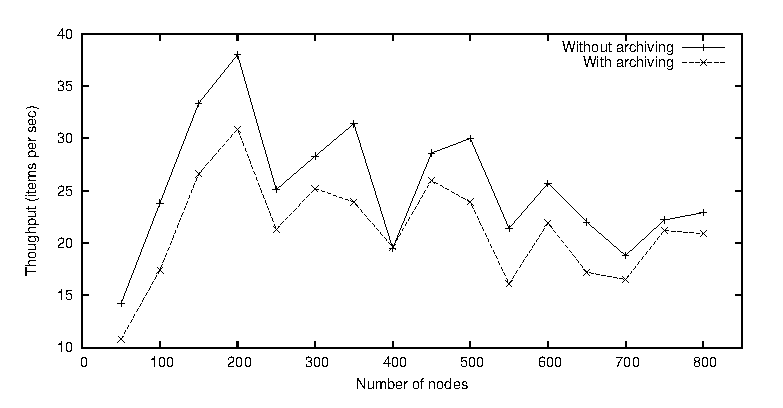
\epsfig{file=throughput.eps, width=\columnwidth}
\caption{Average throughput}
\end{center}
\end{figure}

\begin{figure}
\begin{center}
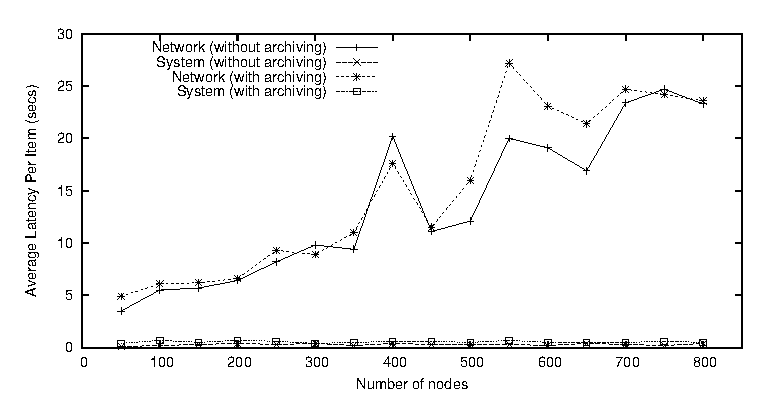
\epsfig{file=latency.eps, width=\columnwidth}
\caption{Average latencies per node}
\end{center}
\end{figure}


\begin{table*}
\begin{center}
\begin{tabular}{|l|r|r|r|r|r|r|r|r|r|r|r|r|}\hline
Num of nodes&	50&	100&	150&	200&	250&	300&	350&	400&	450&	500&	550&	600 \\ \hline\hline
Net latency per node (secs)&	9&	4&	4&	4&	8.6&	5.3&	19.1&	19.5&	14.4&	7.8&	12&	13.3 \\ \hline
Sys latency per node (secs)&	0&	0&	0&	0.3&	0.2&	0.4&	0.3&	0.1&	0.3&	0.4&	0.2&	0.7 \\ \hline
%Total Latency (secs)&	9&	4.04&	4&	4.3&	8.8&	5.8&	19.4&	19.6&	14.7&	8.2&	12.3&	14 \\ \hline
Total fetch time (secs)&	9&	5&	4&	5&	23&	9&	22&	23&	26&	14&	27&	28 \\ \hline	
Throughput (items/sec)&	5.6&	20&	37.5&	40&	10.9&	33.3&	15.9&	17.4&	17.3&	35.7&	20.4&	21.4 \\ \hline
\end{tabular}
\end{center}
\caption{Performance of Comon with no archiving}
\end{table*}


\begin{table*}
\begin{center}
\begin{tabular}{|l|r|r|r|r|r|r|r|r|r|r|r|r|}\hline
Num of nodes&	50&	100&	150&	200&	250&	300&	350&	400&	450&	500&	550&	600 \\ \hline\hline
Net latency per node (secs)&	16&	4&	4&	4&	18.9&	6&	20.6&	22&	8.4&	13&	21.8&	21.3 \\ \hline
Sys latency per node (secs)&	0.8&	1.28&	1.4&	1.8&	1.9&	1.5&	1.6&	1.3&	1.9&	1.7&	1.7&	2.2 \\ \hline
%Total Latency (secs)&	16.8&	5.28&	5.4&	5.8&	20.8&	7.5&	22.2&	23.3&	10.3&	14.7&	23.56&	23.5 \\ \hline
Total fetch time (secs)&	17&	6&	7&	7&	27&	12&	27&	30&	19&	33&	43&	43 \\ \hline
Throughput (items/sec)&	2.9&	16.7&	21.4&	28.6&	9.3&	25&	13&	13.3&	23.7&	15.2&	12.8&	14 \\ \hline
\end{tabular}
\end{center}
\caption{Performance of Comon with archiving}
\end{table*}


\section{Related Work}
\label{sec:related}
\section{Related Work}\label{sec:related}



\section{Conclusions}
\label{sec:conclusions}
The explosive growth of the internet has made monitoring and managing
data systems distributed across wide-area networks increasingly
important.  The possibility of partial failure and the need to
synchronize makes such code tedious and difficult to write correctly,
particularly for data experts whose skills are in domains other than
networking. In this paper, we describe the \padsd{} system, which
allows users to declaratively specify their data systems and then
generate a wide-variety of tools for manipulating the data: from
stand-alone tools, to simple libraries for writing their own analyses,
to generic libraries for building new generic tools.  We precisely
specify the meaning of our language via a sound denotational
semantics and show via experimentation that the system has
acceptable performance overheads.


% \section*{Acknowledgments}

% This material is based upon work 
% supported by the NSF
%    under grants 0612147 and 0615062.
% Any opinions, findings, and conclusions or recommendations
%    expressed in this material are those of the authors and do not
%    necessarily reflect the views of the NSF.

\bibliographystyle{abbrv}
\bibliography{pads,vivek}

%\appendix{}

%\section{Semantics Rewrite -- dpw -- Feb 18, 2009}

A {\em dependency set} is a set of time-location pairs.
Let type $\dsty$ be $\setty{\timety * \locty}$. 
Let $\ds$ range over objects with type $\dsty$.
A {\em schedule} is a set of times.  Let
$\schedulety$ be $\setty{\timety}$.  Let
$\schedule$ range over objects with type $\schedulety$.
({\em Previously, $\schedule$ was an atomic, uninterpreted set of constants in the language.
Previously, sets were not included as a type.}).
Figure~\ref{fig:syntax-revised} contains the revised language 
syntax.

\begin{figure}[t]
\[
\begin{array}{lll}
\multicolumn{3}{l}{\mbox{(host-language base types)}}\\ 
\multicolumn{3}{l}{\basety \ ::= \boolty \bnfalt \stringty \bnfalt \locty \bnfalt \timety} \\
\\
\multicolumn{3}{l}{\mbox{(host-language types)}}\\ 
\multicolumn{3}{l}{\ty \ ::=\ \basety
\bnfalt \optionty{\ty}
\bnfalt \ty_1 * \ty_2
\bnfalt \ty_1 + \ty_2
\bnfalt \listty{\ty}
\bnfalt \setty{\ty}
\bnfalt \ty_1 \arrow \ty_2
} \\
\\
\multicolumn{3}{l}{\mbox{(host-language values)}}\\ 
\multicolumn{3}{l}{\data \ ::=} \\
& \boolf \bnfalt \boolt & \mbox{booleans} \\
\bnfalt & \astring \bnfalt \loc \bnfalt \atime &
 \mbox{strings, locations, times} \\
\bnfalt & \none \bnfalt 
                           \some{\data} & \mbox{optional values}\\
\bnfalt & (\data_1,\data_2) & \mbox{pairs} \\
\bnfalt & \inl{\data} \bnfalt 
                           \inr{\data} & \mbox{sum values} \\
\bnfalt & 
%\nillist \bnfalt 
                           \conslist{\data_1}{\data_n} & \mbox{list values} \\
% & \bnfalt & \nilstream \bnfalt 
%                           \consstream{\data_1}{\data_2} & \mbox{stream values} \\

\bnfalt & \lambda x{:}\ty.\expression & \mbox{function values} \\
\\
\multicolumn{3}{l}{\mbox{(host-language expressions)}}\\ 
\multicolumn{3}{l}{\expression \ ::=}\\ 
& \generalvar & \mbox{variables} \\
\bnfalt & \data & \mbox{data values} \\
\bnfalt & \none \bnfalt 
              \some{\expression} & \mbox{option expressions}\\
%\bnfalt & (\expression_1,\expression_2) \bnfalt e.1 \bnfalt e.2 
%    & \mbox{pair expressions} \\
% & \bnfalt & \inl{\expression} \bnfalt 
%             \inr{\expression} & \mbox{sum expressions} \\
% & \bnfalt & \expression_1 \; \expression_2 & \mbox{application expression} \\
\bnfalt & ... & \mbox{more typed lambda expressions} \\
%\\
%\multicolumn{4}{l}{\mbox{(feed meta-data:  a subset of host language values)}}\\ 
%\multicolumn{4}{l}{\mbox{(a special location (\generatedloc) is used when data is created artificially)}}\\ 
\end{array}
\]
\caption{Host Language Syntax.}
\label{fig:host-language}
\end{figure}


\begin{figure}[t]
\[
\begin{array}{lll}
\multicolumn{3}{l}{\mbox{(feed types)}}\\ 
\multicolumn{3}{l}{\sigma \ ::= \tau \bnfalt \optionty{\tau} 
  \bnfalt \sigma_1 * \sigma_2
  \bnfalt \sigma_1 + \sigma_2
  \bnfalt \listty{\sigma}
}   \\  
\\
\multicolumn{3}{l}{\mbox{(core feed spec)}}\\ 
\multicolumn{3}{l}{\corefeed \ ::= }\\
& \{ \ \mathtt{src=}\    e_1;    & \mbox{source specification} \\
& \ \ \ \mathtt{sched=}\  e_2;    & \mbox{schedule specification}\\
& \ \ \ \mathtt{win=}\    e_3;    & \mbox{time-out window specification} \\
& \ \ \ \mathtt{pp=}\     e_4;    & \mbox{pre-processor} \\
& \ \ \ \mathtt{format=}\ e_5; \} & \mbox{format specification}\\ 
\\
\multicolumn{3}{l}{\mbox{(feed specs)}}\\ 
\multicolumn{3}{l}{\feed \ ::=}   \\  
% & x &  \mbox{feed variable} \\ %% no feed variables now
% & \bnfalt 
         & \mathtt{all}\ \corefeed & \mbox{all sources}\\ 
 \bnfalt & \mathtt{any}\ \corefeed & \mbox{one of multiple sources}\\ 
 \bnfalt & \emptyfeed & \mbox{empty feed} \\
 \bnfalt & \onefeed{e_1}{e_2} & \mbox{singleton feed} \\
 \bnfalt & \sfeed{e} & \mbox{schedule to feed} \\
% \bnfalt & \lfeed{e} & \mbox{list to feed} \\
 \bnfalt & \feed_1 \unionfeed \feed_2 & \mbox{union feed} \\
 \bnfalt & \feed_1 \sumfeed \feed_2 & \mbox{sum feed} \\
 \bnfalt & (\feed_1, \feed_2) & \mbox{pair feed} \\
 \bnfalt & [\feed \bnfalt x \leftarrow e ] & \mbox{list comprehension feed} \\
 \bnfalt & \comprehensionfeed{\feed_2}{x}{\feed_1} & \mbox{feed comprehension} \\
 \bnfalt & \filterfeed{\feed}{e} & \mbox{filter feed} \\
 \bnfalt & \letfeed{x}{e_1}{\feed_2} & \mbox{let feed} \\
% & \bnfalt & \feed_1 cartesian \feed_2 & \mbox{cartesian pair -- use a symbol different from *} \\
% & \bnfalt & \feed_1 * \feed_2 & \mbox{continuous pair} \\
% & \bnfalt & \feed_1 {*}{*} \feed_2 & \mbox{local pair} \\
% \bnfalt & x{:}\feed_1 * \feed_2 & \mbox{dependent continuous pair} \\
% \bnfalt & x{:}\feed_1\, {*}{*} \, \feed_2 & \mbox{dependent local pair} \\
% \bnfalt &     \mathtt{foreach{*}}\; x \; 
%    \mathtt{in}\; \feed_1 & \mbox{for each $x$ create continuous $\feed_2$} \\
% &   \quad \mathtt{create}\; \feed_2 \\
% \bnfalt &     \mathtt{foreach{*}{*}}\; x \; 
%    \mathtt{in}\; \feed_1 & \mbox{for each $x$ update local $\feed_2$}\\
% &   \quad \mathtt{update}\; \feed_2 \\
%\foreachcreate{x}{\feed_1}{\feed_2} & \mbox{for each $x$ create continuous $F_2$} \\
% \bnfalt & \foreachupdate{x}{\feed_1}{\feed_2} & \mbox{for each $x$ create local $F_2$} \\
% & \bnfalt & \ppfeed{\feed}{e} & \mbox{preprocess (eg, unzip) data} \\
% & \bnfalt & \remap{\feed}{e} & \mbox{direct feed to different locations/times} \\
% & \bnfalt & \refeed{\feed}{e} & \mbox{adapt feed to new schedule; 
%                                               fill missing entries with ``None''} \\
% & \bnfalt & \stutterfeed{\feed}{e} & \mbox{stutter on new schedule} \\
\end{array}
\]
\caption{Revised Feed Language Syntax.}
\label{fig:syntax-revised}
\end{figure}

Having talked to Amal on
the phone, I believe the theorem I intend to prove 
is called dependency correctness and
is very, very similar to what James Cheny, Amal Ahmed and Umut Acar
proved in their paper ``Provenance as Dependency Analysis.''
It requires a rewrite of the semantics to fully track the set of time-location
pairs upon which the values in a feed depend. Here is the modified metadata 
definition.  Let $\nested$ range over ``nested'' meta-data and $\meta$ range over
a complete meta-data data structure.

\[
\begin{array}{lcll} 
\nested & ::=     
          & (\atime,\loc,\mathtt{None}) & \mbox{base metadata (timeout)} \\
& \bnfalt & (\atime,\loc,\mathtt{Some}\; \atime) & \mbox{base metadata (success)} \\
& \bnfalt & (\nested_1,\nested_2) & \mbox{pair metadata} \\
& \bnfalt & \inl{\nested} & \mbox{sum metadata} \\
& \bnfalt & \inr{\nested} & \mbox{sum metadata} \\
& \bnfalt & [\nested_1,\ldots,\nested_k] & \mbox{list metadata} \\
\\
\meta & ::= & (\atime,\ds,\nested) & \mbox{complete metadata} \\  
\end{array}
\] 

Given meta-data $\meta$, we write $\mytime{\meta}$, $\myds{\meta}$ and
$\myval{\meta}$ for the first, second and third projections (respectively) of $\meta$.
Note the base metadata is a triple of scheduled time, location of origin 
and optional arrival time where {\tt None} indicates the data did not arrive
in a timely manner.

If the feed typing rules give feed $\feed$ type $\feedty{\sigma}$, 
then its data has type $\sigma$ and
its meta data has type $\metatype{\sigma}$ where $\metatype{\sigma}$ is
defined as follows.

\[
\begin {array} {lcl}
\nestedtype{\ty} & = & \timety * \locty * (\optionty{\timety}) \\
\nestedtype{\optionty{\ty}} & = & \timety * \locty * (\optionty{\timety}) \\
\nestedtype{\sigma_1 * \sigma_2} & = & \nestedtype{\sigma_1} * \nestedtype{\sigma_2} \\
\nestedtype{\sigma_1 + \sigma_2} & = & \nestedtype{\sigma_1} + \nestedtype{\sigma_2} \\
\nestedtype{\listty{\sigma}} & = & \listty{\nestedtype{\sigma}} \\
\\
\metatype{\sigma} & = & \timety * \dsty * \nestedtype{\sigma} \\
\end{array}
\]


The theorem to prove goes as follows.

\begin{definition}[Equal Universes Relative to a Dependency Set]
$\ueq{\universe_1}{\ds}{\universe_2}$ if and only if for all
$(\atime,\loc) \in \ds$, $\universe_1(\atime,\loc) = \universe_2(\atime,\loc)$.
\end{definition}

Let $S_1$, $S_2$ range over denotations of feeds.

\begin{definition}[Feed Subset Relative to a Dependency Set]
$\fsubset{S_1}{\ds}{S_2}$ if and only if for all
$(\meta,v) \in S_1$ such that
$\myds{\meta} \subseteq \ds$, $(\meta,v) \in S_2$.
\end{definition}

\begin{definition}[Feed Equality Relative to a Dependency Set]
$\feq{S_1}{\ds}{S_2}$ if and only if 
$\fsubset{S_1}{\ds}{S_2}$ and
$\fsubset{S_2}{\ds}{S_1}$
\end{definition}

\begin{theorem}[Dependency Correctness]
If $\ueq{\universe_1}{\ds}{\universe_2}$ then
$\feq{\semantics{\feed}{\environment}{\universe_1}}{\ds}{\semantics{\feed}{\environment}{\universe_2}}$
\end{theorem}

The proof of dependency correctness is by induction on the structure of feeds.  I
checked out a couple of cases to see how the proof goes and it seemed plausible to
me that I would be able to prove it completely.   
Then I fleshed out all the rules.  I need to proof-read the rules and then go back
and do the full proof start-to-finish.  However, the proof could definitely
fail for the cases of pairs and lists -- I think those cases will need to be revised,
but as of writing this note (1pm feb 19) I haven't had a chance to go back.  

%Figure~\ref{fig:typing-revised} contains 
We'll naturally also want to keep our type safety theorem, hence we need a slight rewrite of
the typing rules.  Here follows the revised definition of feed typing.

%\begin{figure}[t]

% \[
% \infer[(\textit{t-var})]
% {\Gamma \turn x : \Gamma(x)}
% {}
% \]

\[
\infer[(\textit{t-core})]
{ \begin{array}{l}
  \Gamma \turn 
   \{
      \mathtt{src=} e_1;\
      \mathtt{sched=} e_2; \
      \mathtt{win=} e_3;\\ \qquad \ \ 
      \mathtt{pp=} e_4;\
      \mathtt{ format=} e_5; 
   \} 
   : \corety{\optionty{\ty}}
 \end{array}
}
{
 \begin{array}{c}
  \Gamma \turn e_1 : \listty{\locty} \quad \
  \Gamma \turn e_2 : \schedulety \quad \
  \Gamma \turn e_3 : \timety\\
  \Gamma \turn e_4 : \optionty{\stringty} \arrow \optionty{\stringty}  \\
  \Gamma \turn e_5 : \optionty{\stringty} \arrow \optionty{\ty} \\
 \end{array}
}
\]

\[
\infer[(\textit{t-all})]
{ \begin{array}{l}
  \Gamma \turn \mathtt{all}\ \corefeed{} : \feedty{\sigma}
 \end{array}
}
{
 \begin{array}{c}
  \Gamma \turn \corefeed{} : \corety{\sigma}
 \end{array}
}
\]

\[
\infer[(\textit{t-any})]
{ \begin{array}{l}
  \Gamma \turn \mathtt{any}\ \corefeed{} : \feedty{\sigma}
 \end{array}
}
{
 \begin{array}{c}
  \Gamma \turn \corefeed{} : \corety{\sigma}
 \end{array}
}
\]

\[
\infer[(\textit{t-empty})]
{\Gamma \turn \emptyfeed : \feedty{\sigma}}
{}
\]

\[
\infer[(\textit{t-one})]
{\Gamma \turn \onefeed{e_1}{e_2} : \feedty{\tau}}
{\Gamma \turn e_1 : \tau
 \qquad
 \Gamma \turn e_2 : \timety
}
\]

\[
\infer[(\textit{t-schedule})]
{\Gamma \turn \sfeed{e} : \feedty{\timety}}
{\Gamma \turn e : \schedulety
}
\]


%% \[
%% \infer[(\textit{t-list})]
%% {\Gamma \turn \lfeed{e} : \feedty{\tau}}
%% {\Gamma \turn e : \listty{\tau}
%% }
%% \]

\[
\infer[(\textit{t-union})]
{\Gamma \turn \feed_1 \unionfeed \feed_2  : \feedty{\sigma}}
{
  \Gamma \turn \feed_1 : \feedty{\sigma} &
  \Gamma \turn \feed_2 : \feedty{\sigma}
}
\]

\[
\infer[(\textit{t-sum})]
{\Gamma \turn \feed_1 \sumfeed \feed_2  : \feedty{\sigma_1 + \sigma_2}}
{
  \Gamma \turn \feed_1 : \feedty{\sigma_1} &
  \Gamma \turn \feed_2 : \feedty{\sigma_2}
}
\]

\[
\infer[(\textit{t-pair})]
{\Gamma \turn (\feed_1, \feed_2)  : \feedty{\sigma_1 * \sigma_2}}
{
  \Gamma \turn \feed_1 : \feedty{\sigma_1} &
  \Gamma \turn \feed_2 : \feedty{\sigma_2}
}
\]

\[
\infer[(\textit{t-list})]
{\Gamma \turn [\feed \bnfalt x \leftarrow e ]  : \feedty{\listty{\sigma}}}
{
  \Gamma \turn e : \listty{\tau} &
  \Gamma,x{:}\tau \turn \feed : \feedty{\sigma} 
}
\]

\[
\infer[(\textit{t-comph})]
{\Gamma \turn \comprehensionfeed{\feed_2}{x}{\feed_1} : \feedty{\sigma}}
{
  \Gamma \turn \feed_1 :  \feedty{\sigma} &
  \Gamma,x{:}\metatype{\sigma} * \sigma \turn \feed_2 : \feedty{\sigma} 
}
\]

\[
\infer[(\textit{t-filter})]
{\Gamma \turn \filterfeed{\feed}{e} : \feedty{\sigma}}
{
  \Gamma \turn \feed : \feedty{\sigma} &
  \Gamma \turn e : (\metatype{\sigma} * \sigma) \arrow \boolty
}
\]

\[
\infer[(\textit{t-let})]
{\Gamma \turn \letfeed{x}{e_1}{\feed_2} : \feedty{\sigma_2}}
{
  \Gamma \turn e_1 : \ty_1 & 
  \Gamma,x{:}\ty_1 \turn \feed_2 : \feedty{\sigma_2} 
}
\]

%\caption{Feed Language Typing.}
%\label{fig:typing-revised}
%\end{figure}


Figure~\ref{fig:semantics-revised} contains revised definitions of feeds.


\begin{figure*}[t]
\[
\begin{array}{lcl}

    {\cal C}\lsem\mathtt{\{ src=} e_{src}; 
 &=& \{( \mathtt{meta} (\atime,\loc), \mathtt{val} (\atime,\loc))
          \setalt \atime \in S
          \;\mbox{and}\; \loc \in  L
     \}
\\
 \quad\ \   \mathtt{sched=} e_{sched};
&&\quad\mbox{where} \\
 \quad\ \  \mathtt{win=} e_{win};
&& \qquad S = \esemantics{e_{sched}}{\environment} \\
 \quad\ \  \mathtt{pp=} e_{pp};
&& \qquad W = \esemantics{e_{win}}{\environment}\\
 \quad\ \  \mathtt{format=} e_{f}; \}\rsem_{{\environment} \,
   {\universe}}
&& \qquad L = \esemantics{e_{src}}{\environment}
\\
&& \qquad \mathtt{timeout} =  
     \lambda (x_t,(x_{at},x_s)).
        \mathtt{if}\, x_{at} \leq x_t + W \,
        \mathtt{then}\,  x_s \, \mathtt{else} \, \mathtt{None} 
\\
&& 
\qquad \mathtt{arrival} =  
     \lambda (x_t,(x_{at},x_s)).
        \mathtt{if}\, x_{at} \leq x_t + W \,
        \mathtt{then}\,  \mathtt{Some}\, x_{at} \, \mathtt{else} \, \mathtt{None} 
 \\
&& 
\qquad \mathtt{meta} =  
      \lambda (\atime,\loc).
       (\atime,\{(\atime,\loc)\}, (\atime,\loc,\mathtt{arrival}(\atime,\universe(\atime,\loc))))
\\
 && \qquad \mathtt{val} =
      \lambda (\atime, \loc).
             \esemantics{e_f\; (\universe'(\atime, \loc))}{\environment}
 \\
&& \qquad \universe' =
     \lambda (\atime, \loc). 
           \esemantics{e_{pp}}{\environment}\, 
                 (\mathtt{timeout}\, (\atime,\universe (\atime,\loc))) 

\\



\\\\

\semantics{\mathtt{all}\ \corefeed}{\environment}{\universe} 
&=& 
\csemantics{C}{\environment}{\universe}
\\\\


%New version: any rule
\semantics{\mathtt{any}\ \corefeed}{\environment}{\universe}
& = & \{ i_t\ |\ \atime \in S\}\\
&&
\begin{array}{l}
 \begin{array}{ll@{\hspace{1ex}}c@{\hspace{1ex}}l}
 \mbox{where} & A        & = &\csemantics{C}{\environment}{\universe}\\
              & S        & = & \{\mytime{\meta}\ |\ (\meta, v) \in A\}\\
              & A_\atime & = & \{(\meta,v)\ | \ (\meta, v) \in A\ \mbox{and} \ \mytime{\meta} = \atime\}\\
              & DS_\atime & = & \bigcup_{(\meta,v) \in A_\atime} \myds{\meta} \\
              & V_\atime & = & \{(\meta,\some{v})\ | \ (\meta, \some{v}) \in A_\atime\}\\
              & i_\atime & = & \left\{ \begin{array}{lll}
                                           \mbox{\selectOne}(V_\atime) \; \mbox{with} \; \myds{\meta} = DS_\atime& \mbox{if} & |V_\atime| > 0\\
                                           ((\atime, DS_\atime, (\atime,\generatedloc,\none)), \none) & \mbox{if} & |V_\atime| = 0 \\
                                           \end{array} \right.
 \end{array}
\end{array} 
%%End New version: any rule
\\\\

\semantics{\emptyfeed}{\environment}{\universe} 
 &=& \{\;\}
\\\\
\semantics{\onefeed{e_1}{e_2}}{\environment}{\universe} 
 &=& \{
   ((\esemantics{e_2}{\environment},
    \{\;\}, 
       (\esemantics{e_2}{\environment},\generatedloc,
         \mathtt{Some}\;\esemantics{e_2}{\environment})),
    \esemantics{e_1}{\environment})\}
\\\\
\semantics{\sfeed{e}}{\environment}{\universe} 
 &=& \{((\atime,\{\;\},(\atime,\generatedloc,\mathtt{Some}\; \atime)), \atime) 
          \setalt \atime \in  \esemantics{e}{\environment} 
     \}
\\\\
%% \semantics{\lfeed{e}}{\environment}{\universe} 
%%  &=& \{((\atime,\{\},\generatedloc), \atime) 
%%           \setalt \atime \in  \esemantics{e}{\environment} 
%%      \}
%% \\\\
\semantics{\feed_1 \unionfeed \feed_2}{\environment}{\universe} 
 &=& \semantics{\feed_1}{\environment}{\universe} 
     \bigcup
     \semantics{\feed_2}{\environment}{\universe} 
\\\\
\semantics{\feed_1 \sumfeed \feed_2}{\environment}{\universe} 
 &=& \{
      ((\mytime{\meta},\myds{\meta},\inl{\myval{\meta}}),\inl{v}) \setalt 
        (\meta,v) \in \semantics{\feed_1}{\environment}{\universe} 
     \} \bigcup
 \\
&&
     \{
      ((\mytime{\meta},\myds{\meta},\inr{\myval{\meta}}),\inr{v}) \setalt 
        (\meta,v) \in \semantics{\feed_2}{\environment}{\universe}
     \}
\\\\
\semantics{(\feed_1, \feed_2)}{\environment}{\universe} 
 &=&
 \{((\mytime{\meta_1},\myds{\meta_1}\cup\myds{\meta_2}, (\myval{\meta_1},\myval{\meta_2})),(v_1,v_2)) 
  \setalt 
\\
&& \quad
     (\meta_1,v_1) \in \semantics{\feed_1}{\environment}{\universe} 
     \; \mbox{and} \; 
     (\meta_2,v_2) \in \semantics{\feed_2}{\environment}{\universe}
     \; \mbox{and} \; 
     \mytime{\meta_1} = \mytime{\meta_2}
  \}
\\\\
\semantics{[\feed \bnfalt x \leftarrow e]}{\environment}{\universe} 
 &=&
 \{((\atime,\bigcup_{i=1\ldots{}k} \myds{\meta_i}, [\myval{\meta_1},\ldots,\myval{\meta_k}]),[v_1,\ldots,v_k]) \setalt 
\\ && \quad
    \forall i:1\ldots k.
     (\meta_i,v_i) \in \semantics{\feed}{(\environment,x\mapsto z_i)}{\universe} 
     \; \mbox{and} \; 
     \mytime{\meta_i} =\atime
  \} \\
&&\quad\mbox{where} \quad\mbox{$[z_1,\ldots,z_k] = \esemantics{e}{\environment}$}
\\\\
\semantics{\comprehensionfeed{\feed_2}{x}{\feed_1}}{\environment}{\universe} 
 &=& \{((\mytime{\meta_2},\myds{\meta_1} \cup \myds{\meta_2}, \myval{\meta_2}),v_2) 
          \setalt (\meta_1, v_1) \in  \semantics{\feed_1}{\environment}{\universe} \; \mbox{and} \;
          (\meta_2,v_2) \in \semantics{\feed_2}{(\environment,x\mapsto(\meta_1,v_1))}{\universe}  
     \} 
\\\\
\semantics{\filterfeed{\feed}{e}}{\environment}{\universe} 
 &=&
\{(\meta,v) \setalt (\meta,v) \in \semantics{\feed}{\environment}{\universe} \; \mbox{and} \;
            \esemantics{e \; (\meta,v)}{\environment} = \mathtt{true}
\}
\\\\
\semantics{\letfeed{x}{e_1}{\feed_2}}{\environment}{\universe} 
 &=& \semantics{\feed_2}{(\environment,x\mapsto\esemantics{e_1}{\environment})}{\universe} 
\\
\end{array}
\]
\caption{Feed Language Semantics.}
\label{fig:semantics-revised}
\end{figure*}


\end{document}

%%% Local Variables:
%%% mode: outline-minor
%%% End:

